\documentclass[tikz,12pt,margin=0px]{article}

\usepackage[a4paper,bindingoffset=0.2in,
            left=1.5cm,right=1.5cm,top=1.25cm,bottom=1.5cm,%
            footskip=.3in]{geometry}
\usepackage[normalem]{ulem}
\usepackage[utf8]{inputenc}
\usepackage{amsmath}
\usepackage{amssymb}
\usepackage{comment}
\usepackage{color, colortbl}
\usepackage[dvipsnames]{xcolor}
\usepackage{dsfont}
\usepackage{enumitem}
\usepackage{multirow}
\usepackage{fancyhdr}
\usepackage{float}
\usepackage{fontawesome}
\usepackage{makecell}
\usepackage{tikz}
\usepackage{titlesec}
\usepackage[hungarian]{babel}
\usetikzlibrary{positioning,calc,shapes.multipart,arrows,arrows.meta,matrix,automata,shapes.misc,er}

\setlist[itemize,1]{label=$\bullet$}
\setlist[itemize,2]{label=$\circ$}
\setlist[itemize,3]{label=$\centerdot$}
\setlist[itemize,4]{label=$\cdot$}

\titleformat*{\section}{\Large\bfseries}
\titleformat*{\subsection}{\large\bfseries}
\titleformat*{\subsubsection}{\normalsize\bfseries}
\titleformat*{\paragraph}{\small\bfseries}
\titleformat*{\subparagraph}{\footnotesize\bfseries}

\pagestyle{fancy}

\newcommand\blfootnote[1]{%
  \begingroup
  \renewcommand\thefootnote{}\footnote{#1}%
  \addtocounter{footnote}{-1}%
  \endgroup
}

\renewcommand{\figurename}{ábra}
\newenvironment{tetel}[1]{\paragraph{#1 \\}}{}

\newcommand{\N}{\mathbb{N}}
\newcommand{\Z}{\mathbb{Z}}
\newcommand{\R}{\mathbb{R}}
\newcommand{\Q}{\mathbb{Q}}
\newcommand{\C}{\mathbb{C}}

\makeatletter
\renewcommand\paragraph{%
	\@startsection{paragraph}{4}{0mm}%
	{-\baselineskip}%
	{.5\baselineskip}%
	{\normalfont\normalsize\bfseries}}
\makeatother

\newcommand\lword[1]{\leavevmode\nobreak\hskip0pt plus\linewidth\penalty50\hskip0pt plus-\linewidth\nobreak #1}

\useunder{\uline}{\ul}{}
\fancyhead{}
\cfoot{18. tétel | \thepage. oldal}

\renewcommand{\headrulewidth}{0pt}
\renewcommand{\footrulewidth}{0.4pt}

\tikzstyle{line} = [draw,thick]

\colorlet{notgray}{gray!20!white}
\colorlet{notblue}{green!25!white}
\colorlet{notgreen}{green!10!white}
\newcolumntype{g}{>{\columncolor{notgray}}c}
\newcolumntype{b}{>{\columncolor{notblue}}c}
\newcolumntype{e}{>{\columncolor{notgreen}}c}

\begin{document}
    \thispagestyle{fancy}
    \hyphenation{oddword}
    \uchyph=0

    \begin{center}
        {\Large\bfseries\noindent 18. Adatbázisok tervezése és lekérdezése} \\
    \end{center}
	
	\section*{Relációs adatmodell, egyed-kapcsolat modell és átalakítása relációs adatmodellbe}
	
	\subsection*{Relációs adatmodell\\}
	
    \textbf{Adatmodell}: Egy adatmodell a valóság objektumait (egyedeit), azok tulajdonságait, ill. a köztük lévő kapcsolatokat ábrázolja. Az adatmodell a számítógép és felhasználó számára is megadja, hogy hogyan néznek ki az adatok. Az adatok leírására szolgáló jelölés, melynek részei:

    \begin{itemize}
        \item \textbf{az adat struktúrája} (\emph{statikus elemek})
        \item \textbf{az adaton végezhető műveletek} (\emph{dinamikus elemek})
        \item \textbf{az adatokra tett megszorítások} (\emph{integritási feltételek)}\\
        {\small Például: egy személyi igazolvány számhoz nem tartozhat két különböző ember}
    \end{itemize}

   \noindent \textbf{Relációs adatmodell}: A relációs adatmodellben egy adatbázis kétdimenziós adattáblák összessége, ahol minden adattábla egy reláció vagyis sorok (rekordok) halmaza.\\
	
    \noindent \textbf{Reláció}: Az adatelemek megnevezett, összetartozó csoportjából kialakított olyan kétdimenziós táblázat, amelyik sorokból (rekordok) és oszlopokból (attribútumok) áll. A relációnak egyedi neve van és oszlopait az attribútumok címzik. A reláció rekordjait tetszőlegesen megcserélhetjük, sorok sorrendje lényegtelen (a halmazszemlélet miatt).\\

    \noindent \emph{Formálisan}: Legyenek $H_{1}, \ldots, H_{n}$ alaphalmazok, akkor $r \subset H_{1} \times \ldots \times H_{n}$ részhalmazt relációnak nevezzük.\\

    \noindent \textbf{Attribútumok}: A reláció fejrészében találhatóak az attribútumok. Minden attribútumhoz tartozik egy értékkészlet, amelyből felveheti értékeit. Az $i$-edik attribútum értékkészletét $dom(A_i)$ jelöli.\\

    \noindent Adattípus vagy \emph{sortípus}:
    \begin{center}
        $\big<\textit{attr.név}_1 : \text{értéktípus}_1,\ \ldots,\ \textit{attr.név}_{n} : \text{értéktípus}_{n}\big>$, ahol $\text{attr.név}_{i} \boldsymbol{\neq} \text{attr.név}_{j}\quad (\forall i \neq j)$.\\
    \end{center}

    \noindent A reláció nevét és a reláció attribútumainak halmazát együtt nevezzük \emph{\textbf{relációsémának}}.\\
    \noindent \emph{Relációséma}: \textbf{\emph{Relációnév(sortípus)}}, azaz
    \begin{center}
        $R(\textit{attr.név}_1 : \text{értéktípus}_1, \ldots, \textit{attr.név}_{n} : \text{értéktípus}_{n})$\\
        $\Updownarrow$\\
        $R(A_{1}, \ldots, A_{n}) \Leftrightarrow R(U),\ U = \big\{A_{1}, \ldots, A_{n}\big\}$.
    \end{center}

    \noindent A relációs modellben az adatbázis egy vagy több relációsémát tartalmaz. A relációsémákból álló halmazt az adatbázisban \emph{\textbf{relációs adatbázissémának}} vagy röviden \emph{\textbf{adatbázissémának}} nevezzük.\\

    \noindent Adatbázis séma jelölése: $\mathds{R}$, ahol $\mathds{R} = \{R_1 , ... , R_k\}$.

\newpage
    \paragraph*{Relációs séma feletti reláció előfordulás (példány, instance)}

    A reláció azon sorait, amelyek különböznek az attribútumokból álló fejléc soraitól, \emph{\textbf{sor}}oknak (tuple) nevezzük. A reláció minden egyes attribútumához tartozik a sorban egy \emph{komponens}.\\

    \noindent Egy reláció előfordulásainak halmaza a sor-típusnak megfelelő véges sok sor (sorok halmaza), azaz
    \[
        {t_1, \ldots , t_n}\ \text{ahol}\ t_i\ \text{(tuple, sor, rekord)}\quad (i = 1, \ldots, n)\quad \text{(véges sok)}
    \]

    \noindent  Mit jelent egy konkrét sor (rekord)?
    \begin{center}
        $t_{i}: <A_1: \text{érték}_{i,1}, \ldots, A_m:\ \text{érték}_{i,m}>,\ \text{ahol}\ \text{érték}_{i, j} \in dom(A_{j}) \quad (i \in 1, \ldots, n,\ j \in 1, \ldots, m)$
    \end{center}
    \begin{itemize}
        \item \emph{n} - számosság (sorok (rekordok) száma)
        \item \emph{m} - dimenzió (oszlopok (attribútumok) száma)
    \end{itemize}

 	\begin{figure}[H]
 		\centering
 		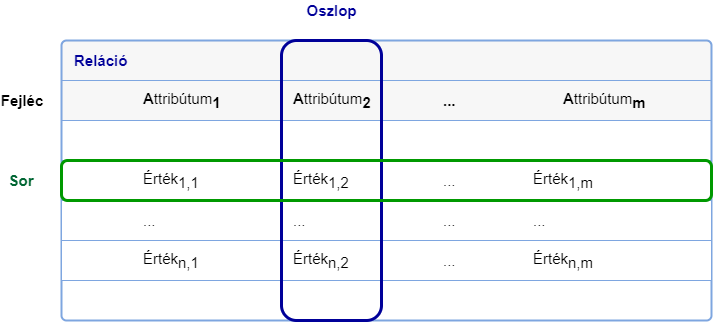
\includegraphics[width=0.66\textwidth]{img/table_relation.png}
% 		\caption{PSM kurzor ciklusának szerkezete}
 	\end{figure}

    \noindent Az attribútumok sorrendje nem rögzített a relációsémában. Azonban egy-egy előfordulás ábrázolása esetén viszont rögzítésre kerül.\\

    \noindent A relációs modellben követelmény, hogy minden sor minden komponense atomi, azaz elemi típusú legyen (például egész vagy karaktersorozat).\\

    \noindent \paragraph*{Kulcsok\\}

    \noindent A $K \subseteq \{A_1, \ldots, A_n\}$ attribútumhalmazt, amelyre az $r \in R(A_1, \ldots, A_n)$ reláció minden sorára különböző \emph{\textbf{szuperkulcs}}nak nevezzük:
    \[
        \forall t_i, t_j \in r,\ i \neq j : t_1[K] \neq t_2[K]
    \]

    \noindent A $K$ attribútumhalmazt \emph{\textbf{kulcs}}nak nevezzük, ha minimális szuperkulcs.\\
%    \begin{enumerate}
%        \item Ezek az attribútumok funkcionálisan meghatározzák a reláció minden más attribútumát, azaz nincs az $R$-ben két olyan különböző sor, amely mindegyik $A_1, \ldots, A_{n}$-en megegyezne.
%        \item Nincs olyan valódi részhalmaza $\{A_1, \ldots, A_{n}\}$-nek, amely funkcionálisan meghatározná az $R$ összes többi attribútumát, azaz a kulcsnak minimálisnak kell lennie.
%    \end{enumerate}

    \noindent Egy relációsémában több kulcs is előfordulhat, vagyis több attribútumhalmazt is ki tudunk jelölni kulcsként.

    \begin{itemize}
        \item A kulcs egy attribútumból áll: \textbf{\emph{egyszerű kulcs}}
        \item A kulcsot több attribútum alkotja: \textbf{\emph{összetett kulcs}}.
        \begin{itemize}
            \item Ha több kulcs is meghatározható a sémában, akkor kijelöljük az egyiket, amelyet \textbf{\emph{elsődleges kulcs}}nak nevezünk.
        \end{itemize}
    \end{itemize}
\newpage
    \noindent \textbf{Külső vagy idegen kulcs}: Ha egy attribútum egy másik séma elsődleges kulcsára hivatkozik.
        \begin{itemize}
            \item $R(A_1,...A_m)$ reláció, és $X=\{A_{i_1},...A_{i_k}\}$ kulcs.
            \item $S(B_1,...B_n)$ reláció, és $Y=\{B_{j_1},...B_{j_k}\}$ idegen kulcs.
            \item Az $Y$ az $X$-re hivatkozik a megadott attribútum sorrendben: $B_{j_1} \to A_{i_1}$-re, és így tovább.\\
        \end{itemize}

	\noindent \textbf{Hivatkozási épség}: Megszorítás a két tábla együttes előfordulására.\\
    Ha $s \in R_1$ sor, akkor $\exists t \in R_2$ sor, amelyre
    \[
        s[B_{j_1},...B_{j_k}] = t[A_{i_1},...A_{i_k}]
    \]

    {\small
    \noindent A relációs adatmodell több szempontból is előnyös, amik miatt elterjedt és kifinomult.
        \begin{itemize}
            \item Az adatmodell egy egyszerű és könnyen megérthető strukturális részt tartalmaz.
            \item A természetes táblázatos formát nem kell magyarázni, és jobban alkalmazható.
            \item A relációs modellben a fogalmi-logikai-fizikai szint teljesen szétválik, nagyfokú logikai és fizikai adatfüggetlenség.
            \item A felhasználó magas szinten, hozzá közel álló fogalmakkal dolgozik (implementáció rejtve).
            \item Elméleti megalapozottság, több absztrakt kezelő nyelv létezik, például relációs algebra\\
            (ezen alapul az SQL automatikus és hatékony lekérdezés optimalizálása).
            \item Műveleti része egyszerű kezelői felület, szabvány SQL.
        \end{itemize}	
    }

	\subsection*{Egyed-kapcsolat (E/K) modell\\}
	
    \noindent Grafikus ábrázolási mód, amellyel egy-egy adatbázis sémája megtervezhető. Az egyed-kapcsolat modellben az adatok szerkezetét grafikusan, egyedkapcsolat diagramon ábrázoljuk. Az így elkészített ábra később könnyen átalakítható relációs adatmodellé. \\

    \noindent A diagram elemei:
    \begin{itemize}
        \item egyedhalmazok
        \item attribútumok
        \item kapcsolatok\\
    \end{itemize}

    \noindent \textbf{\emph{Egyed}}: Az a valami, dolog, amit ismeretekkel akarunk leírni; valami ami van és megkülönbözhető. Az egyedek a valóság azon elemei, melyek számunkra valamilyen lényeges információt hordoznak, \emph{egymástól megkülönböztethetők}.\\

	\noindent \textbf{\emph{Egyedhalmazok}}: Hasonló egyedek összessége. Diagrammon: \emph{téglalap}.\\

    \begin{center}
        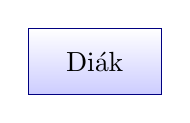
\begin{tikzpicture}[auto,node distance=1.5cm]
            \node[entity] (node1) [top color=white, bottom color=blue!20, draw=blue!50!black!100] {Diák};
        \end{tikzpicture}\\
    \end{center}
\newpage
    \noindent \textbf{\emph{Tulajdonság}} (\emph{attribútum}): A tulajdonság az, amivel az egyedet leírjuk, ami alapján az egyedhalmaz egyedei megkülönböztethetőek a többi egyedtől. A tulajdonság egy konkrét értéke a tulajdonság előfordulása. A tulajdonság előfordulások összességét \lword{tulajdonsághalmaznak} nevezzük. Az attribútumok atomiak, tehát nincs belső szerkezetük. Diagrammon: \emph{ovális}.\\

    \begin{center}
        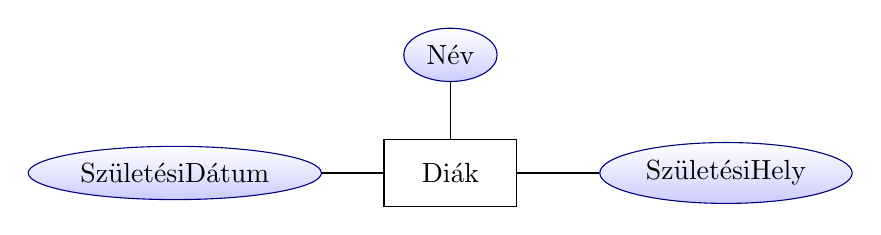
\begin{tikzpicture}[auto,node distance=1.5cm]
            \tikzstyle{every attribute} = [top color=white, bottom color=blue!20, draw=blue!50!black!100]
          \node[entity] (node1) {Diák}
            child {node[attribute] (name) [above of=node1] {Név}}
            child {node[attribute] (birthdate) [left of=node1,node distance=3.5cm]{SzületésiDátum}}
            child {node[attribute] (birthplace) [right of=node1,node distance=3.5cm] {SzületésiHely}};
        \end{tikzpicture}
    \end{center}

    \noindent \emph{Összetett tulajdonság} (\emph{attribútum}): Olyan tulajdonság, amelynek magának is vannak tulajdonságai.

    \begin{center}
        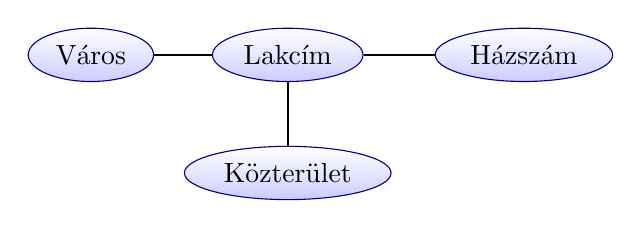
\begin{tikzpicture}[auto,node distance=1.5cm]
            \tikzstyle{every attribute} = [top color=white, bottom color=blue!20, draw=blue!50!black!100]
          \node[attribute] (attr1) {Lakcím};
          \node[attribute, node distance=2.5cm] (cityattr) [left of= attr1] {Város};
          \node[attribute, node distance=1.5cm] (streetattr) [below of=attr1]{Közterület};
          \node[attribute, node distance=3.0cm] (placenumberattr) [right of=attr1] {Házszám};
          \path [line] (attr1) -- (cityattr);
          \path [line] (attr1) -- (streetattr);
          \path [line] (attr1) -- (placenumberattr);
        \end{tikzpicture}
    \end{center}

    \noindent \emph{Többértékű tulajdonság}: nem egyetlen adat jellemzi a tulajdonságot, hanem adatok halmaza (sorrendiség nélkül) vagy listája (sorrend számít).

    \begin{center}
        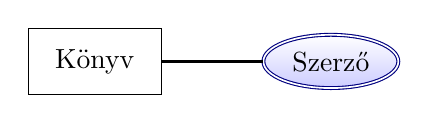
\begin{tikzpicture}[auto]
            \tikzstyle{every attribute} = [top color=white, bottom color=blue!20, draw=blue!50!black!100]
          \node[entity] (node1) {Könyv};
          \node[attribute, node distance=3.0cm, double] (author) [right of=node1] {Szerző};
          \path[line] (node1) -- (author);
        \end{tikzpicture}
    \end{center}

	\noindent \textbf{\emph{Séma}}: $E(A_1,...A_n)$ egyedhalmaz séma ahol:
    \begin{itemize}
        \item $E$ név,
        \item $A_i$ tulajdonság (attribútumok),
        \item $dom(A_i)$ a lehetséges értékek halmaza.
    \end{itemize}

    \noindent \textbf{\emph{Előfordulás}}: $E(A_1,...A_n)$ egyedhalmaz séma egy előfordulása $E=\{e_1,\ldots,e_m\}$
    \begin{itemize}
        \item $e_i(k) \in dom(A_k)$ az egyedek halmaza.
        \item Semelyik két egyed nem egyezik meg minden attribútumán $\to$ (vagyis az összes tulajdonság szuperkulcsot alkot), minimális szuperkulcs = kulcs.
    \end{itemize}

    \noindent \textbf{\emph{Kapcsolatok}}: Kapcsolat két vagy több egyedhalmazt köthet össze egymással. A kapcsolatok tulajdonképpen egyedosztályok előfordulásai közötti relációk. A kapcsolatokat elláthatjuk névvel és a tartozhatnak hozzá attribútumok is. Diagrammon: \emph{rombusz}.
    \begin{itemize}
        \item $K(E_1,\ldots, E_{k}, A_1, \ldots, A_n)$ egy kapcsolat sémája, ahol:
        \begin{itemize}
            \item $K$ a kapcsolat neve,
            \item $E_i$ az egyedhalmazok sémái,
            \item $A_1, \ldots, A_n$ a kapcsolathoz tartozó attribútumok
        \end{itemize}
        \item Ha $k=2$, akkor bináris kapcsolatról, $k > 2$ esetén többágú kapcsolatról beszélünk.
        \item $K(E_1, \ldots,E_p)$ sémájú kapcsolat előfordulása, $K=\{(e_1, \ldots, e_p)\}$ egyed $p$-esek halmaza, ahol $e_i \in E_i$. A kapcsolat előfordulásaira tett megszorítások határozzák meg a kapcsolat típusát.
    \end{itemize}

    \noindent \textbf{\emph{Kapcsolat attribútum}}: A kapcsolattípusoknak is lehetnek attribútumaik, amelyek hasonlóak az egyedtípusokéihoz. A kapcsolat attribútuma a két egyedhalmaz együttes függvénye, de egyiké sem külön.

	\subsection*{Kapcsolatok típusai}

	\begin{itemize}
        \item \emph{\textbf{egy-egy} (1:1)}: Egy $E_1$-beli egyedhez pontosan egy $E_2$-beli egyed tartozhat és fordítva.\\
        {\small Például: Ha a magyar nők és a magyar férfiak közötti jogi értelemben vett érvényes házastársi kapcsolatot szeretnénk modellezni, akkor egy-egy kapcsolatot kell alkalmaznunk.}
        \begin{center}
            \begin{tikzpicture}[auto,node distance=1.5cm]
                \tikzstyle{every node} = [top color=white, bottom color=blue!20, draw=blue!50!black!100]
            \node[relationship] (joins) [right = of node1] {házasság} (node1);
            \node[entity] (pgroup1) [right = of joins] {Férj} edge [<-, line width=1pt] (joins);
            \node[entity] (pgroup2) [left = of joins] {Feleség} edge [<-, line width=1pt] (joins);
            \end{tikzpicture}
        \end{center}
        \item \emph{\textbf{egy-sok} (1:n)}: Minden $E_2$-beli egyedhez legfeljebb $E_1$-beli egyed kapcsolódik, de egy $E_1$-beli egyedhez több $E_2$-beli egyed kapcsolódhat.\\
        {\small Például: Egy anyának egy vagy több gyermeke is lehet, de egy gyermeknek csak és kizárólag egy vér szerinti anyukája lehet.}
        \begin{center}
            \begin{tikzpicture}[auto,node distance=1.5cm]
                \tikzstyle{every node} = [top color=white, bottom color=blue!20, draw=blue!50!black!100]
            \node[relationship] (joins) [right = of node1] {gyermeke} (node1);
            \node[entity] (pgroup1) [right = of joins] {Gyerek} edge [-, line width=1pt] (joins);
            \node[entity] (pgroup2) [left = of joins] {Anya} edge [<-, line width=1pt] (joins);
            \end{tikzpicture}
        \end{center}

        \item \emph{\textbf{sok-sok} (n:m)}: Minden $E_1$-beli egyedhez több $E_2$-beli egyedek egy halmazát rendelhetjük és fordítva. Ha sok-sok kapcsolat van $E_1$ és $E_2$ egyedhalmazok között, akkor $E_1$-et egyenes vonallal kötjük össze $E_2$-vel.\\
            {\small Például: Egy diák több nyelvet is tanulhat, valamint egy nyelvet több diák is tanulhat.}
        \begin{center}
            \begin{tikzpicture}[auto,node distance=1.5cm]
                \tikzstyle{every node} = [top color=white, bottom color=blue!20, draw=blue!50!black!100]
            \node[relationship] (joins) [right = of node1] {tanul} (node1);
            \node[entity] (pgroup1) [right = of joins] {Nyelv} edge [-, line width=1pt] (joins);
            \node[entity] (pgroup2) [left = of joins] {Diák} edge [-, line width=1pt] (joins);
            \end{tikzpicture}
        \end{center}
        \end{itemize}

    \subsubsection*{Speciális kapcsolatok}

    \begin{itemize}
        \item \emph{Önamagára mutató kapcsolat}: Elképzelhető, hogy valamilyen oknál fogva egy egyed önmagával is kapcsolatban állhat, például: dolgozó és főnöke, hiszen a főnök is egy dolgozó, vagy sportoló és edzője, hiszen az edző is egy sportoló.
        \begin{center}
            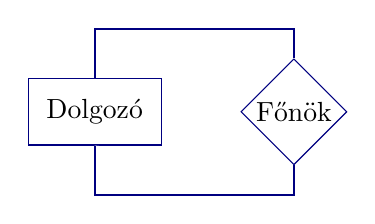
\begin{tikzpicture}[auto,node distance=1.0cm]
                \tikzstyle{every path} = [top color=white, draw=blue!50!black!100]
                \node[entity] (pgroup1) {Dolgozó};
                \node[relationship] (pgroup2) [right = of pgroup1]  {Főnök};
                \path [line] (pgroup1) -- ++(0,-30pt) -| (pgroup2);
                \path [line] (pgroup2) -- ++(0,+30pt) -| (pgroup1);
                % node[transition,pos=0.83,left] {$p_{repl}$};
            \end{tikzpicture} \qquad \qquad
            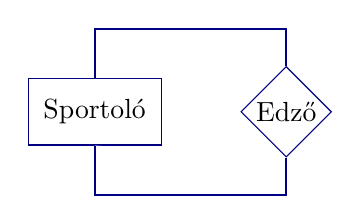
\begin{tikzpicture}[auto,node distance=1.0cm]
                \tikzstyle{every path} = [top color=white, draw=blue!50!black!100]
                \node[entity] (pgroup1) {Sportoló};
                \node[relationship] (pgroup2) [right = of pgroup1]  {Edző};
                \path [line] (pgroup1) -- ++(0,-30pt) -| (pgroup2);
                \path [line] (pgroup2) -- ++(0,+30pt) -| (pgroup1);
                % node[transition,pos=0.83,left] {$p_{repl}$};
            \end{tikzpicture}
        \end{center}
        \item \textbf{\textit{Alosztály} (,,isa"-,,az-egy")}: Gyakran előfordul, hogy egy egyedhalmaz egyedei között egyeseknek olyan speciális tulajdonságaik vannak, amelyekkel nem rendelkezik a halmaz minden egyede. Így célszerű speciális egyedhalmazokat, ún. alosztályokat definiálni, ahol minden alosztálynak vannak speciális attribútumai és/vagy kapcsolatai. \\

            \noindent Ha egy egyedhalmazt alosztályival speciális kapcsolat köt össze, azt "az-egy" (angolul isa) kapcsolatnak nevezzük (például "egy A az egy B" állítás kifejezi a speciális "az-egy" kapcsolatot A-ból B-be). Az öröklési (az-egy) kapcsolatot a hagyományostól eltérően háromszöggel jelöljük, ezzel is kifejezve e kapcsolattípus különlegességét. A háromszög egyik oldalát az alosztállyal kötjük össze, ellenkező oldali csúcsát pedig az ősosztállyal (szuperosztállyal). Minden öröklési kapcsolat egy-egy kapcsolat, de az ezt kifejező nyilakat nem tüntetjük fel külön a diagramon.
        \begin{center}
            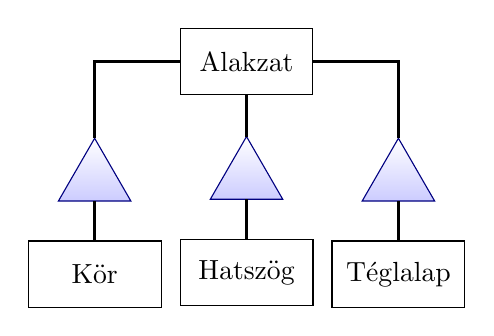
\begin{tikzpicture}[auto,node distance=1.25cm,
            amp/.style = {regular polygon, regular polygon sides=3,
              draw, text width=0.5em,
              inner sep=1mm, outer sep=0mm}]
            \node[entity] (node1) {Alakzat};
            \node[amp] (amp1) [amp, node distance=1.25cm, below left = of node1,top color=white, bottom color=blue!20, draw=blue!50!black!100] {};
            \node[amp] (amp2) [amp, node distance=0.525cm, below = of node1,top color=white, bottom color=blue!20, draw=blue!50!black!100] {};
            \node[amp] (amp3) [amp, node distance=1.25cm, below right = of node1,top color=white, bottom color=blue!20, draw=blue!50!black!100] {};
            \path [line, line width=1pt] (node1) -- ++(-28.8pt,0pt) -| (amp1);
            \path [line, line width=1pt] (node1) -- ++(0,-20pt) -| (amp2);
            \path [line, line width=1pt] (node1) -- ++(+28.8pt,0pt) -| (amp3);
            \node[entity, node distance=0.5cm] (node2) [below = of amp1] {Kör};
            \node[entity, node distance=0.5cm] (node3) [below = of amp2, node distance=1.25cm] {Hatszög};
            \node[entity, node distance=0.5cm] (node4) [below = of amp3, node distance=1.25cm] {Téglalap};
            \path [line, line width=1pt] (amp1) -- ++(0pt,-10pt) -| (node2);
            \path [line, line width=1pt] (amp2) -- ++(0,-10pt) -| (node3);
            \path [line, line width=1pt] (amp3) -- ++(0pt,-10pt) -| (node4);
            \end{tikzpicture}
        \end{center}
	\end{itemize}

    \subsubsection*{Kulcsok}

    \noindent \textbf{Szuperkulcs}: Az egyedhalmaz szuperkulcsa egy azonosító, vagyis olyan tulajdonság-halmaz, amelyről feltehető, hogy az egyedhalmaz előfordulásaiban nem szerepel két különböző egyed, amelyek ezeken a tulajdonságokon megegyeznek. Az összes tulajdonság mindig szuperkulcs.\\

    \noindent \textbf{Kulcs}: Ha attribútumok egy halmaza kulcsot alkot egy egyedhalmazon belül, akkor nincs két olyan egyed, amely megegyezik a kulcs összes attribútumán. Diagrammon: \emph{attribútumnév aláhúzásával}.\\
    \begin{center}
        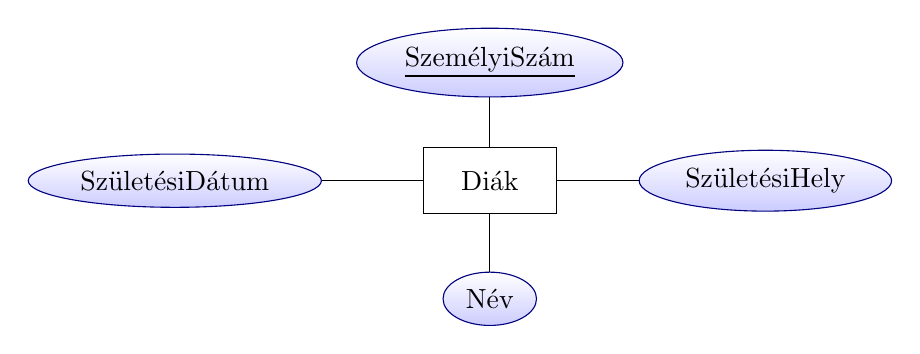
\begin{tikzpicture}[auto,node distance=1.5cm]
            \tikzstyle{every attribute} = [top color=white, bottom color=blue!20, draw=blue!50!black!100]
          \node[entity] (node1) {Diák}
            child {node[attribute] (identitynumber) [above of=node1] {\underline{SzemélyiSzám}}}
            child {node[attribute] (name) [below of=node1] {Név}}
            child {node[attribute] (birthdate) [left of=node1,node distance=4.0cm]{SzületésiDátum}}
            child {node[attribute] (birthplace) [right of=node1,node distance=3.5cm] {SzületésiHely}};
        \end{tikzpicture}
    \end{center}

    \noindent \textit{Megjegyzés}: Jelölhető több kulcs úgy is, hogy megadunk egy kulcsot, ami elsődleges kulcs lesz (ezt úgy kezeljük, mint ha több kulcs nem is lenne) és a többi kulcsot, vagy ne mis jelöljük vagy megjegyzésben felsoroljuk azokat.\\

    \noindent \textbf{Hivatkozási épség}: Azt a követelményt fejezi ki, hogy egy egyedhalmaz egy vagy több attribútumának az értéke elő kell, hogy forduljon egy másik egyedhalmaz adott attribútumának értékeként. Diagrammon: \emph{kerek végű nyíl}.\\

    \noindent \emph{Példa}:

    \begin{center}
        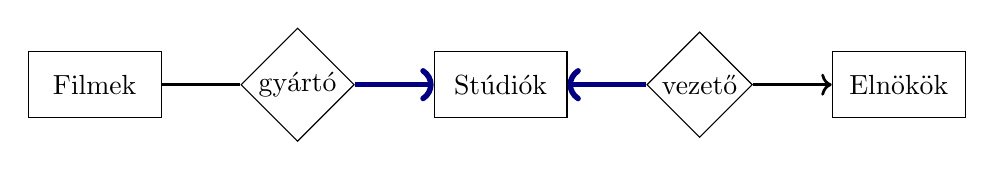
\begin{tikzpicture}[auto,node distance=1.0cm]
            \node[entity] (pgroup1) {Stúdiók};
            \node[relationship] (joins1) [left = of pgroup1] {gyártó};
            \path[top color=white, bottom color=blue!20, draw=blue!50!black!100,line width=2pt] (pgroup1) edge [(-] (joins1);
            \node[relationship] (joins2) [right = of pgroup1] {vezető};
            \path[top color=white, bottom color=blue!20, draw=blue!50!black!100,line width=2pt] (pgroup1) edge [(-] (joins2);
            \node[entity] (pgroup2) [left = of joins1] {Filmek} edge [-, line width=1pt] (joins1);
            \node[entity] (pgroup3) [right = of joins2] {Elnökök} edge [<-, line width=1pt] (joins2);
        \end{tikzpicture}
    \end{center}

    \begin{itemize}
        \item \noindent A \emph{Stúdiók} egyedhalmazhoz megy egy kerek nyíl a \emph{gyártó} kapcsolatban. Ez azt jelenti, hogy annak a stúdiónak, amely gyártott egy filmet, mindig benne kell lennie a \emph{Stúdiók} egyedhalmazban.
        \item Hasonlóan a \emph{Stúdiók} egyedhalmazhoz megy egy kerek nyíl a \emph{vezető} kapcsolatban. Ez azt jelenti, hogy ha egy elnök vezetője egy stúdiónak, akkor annak a stúdiónak léteznie kell a \emph{Stúdiók} egyedhalmazban.
    \end{itemize}

    \paragraph*{Gyenge egyedhalmaz\\}

    \noindent Előfordulhat, hogy egy-egy egyedhalmazt csak más egyedhalmazok attribútumainak ismeretében azonosíthatunk egyértelműen. Ezeket gyenge egyedhalmazoknak nevezzük. A gyenge egyedhalmaz az „azonosító” egyedhalmazokhoz egy-sok kapcsolattal kapcsolódhat.\\

    \noindent Diagrammon:
    \begin{itemize}
        \item \emph{dupla téglalap} az egyedhalmaznak és
        \item \emph{dupla rombusz} azoknak a kapcsolatoknak, amiken keresztül megy az azonosítás.\\
    \end{itemize}

    {\small \emph{Példa gyenge egyedhalmazra}:
    \begin{center}
        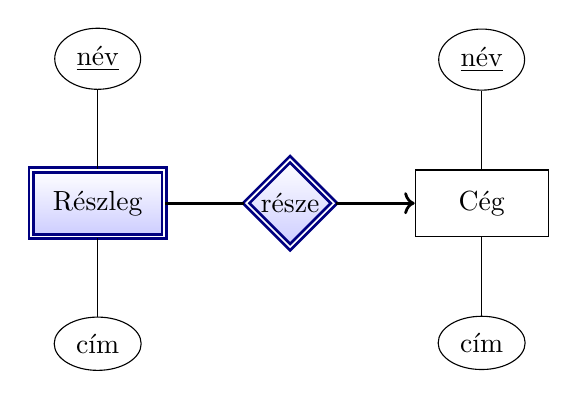
\begin{tikzpicture}[auto,node distance=1.0cm]
           \node[entity, double, top color=white, bottom color=blue!20, draw=blue!50!black!100,line width=1pt] (pgroup1) {Részleg};
           \node[attribute] (oname) [above = of pgroup1] {\underline{név}} edge [-] (pgroup1);
           \node[attribute] (oaddress) [below = of pgroup1] {cím} edge [-] (pgroup1);
           \node[relationship, double, top color=white, bottom color=blue!20, draw=blue!50!black!100,line width=1pt] (joins1) [right = of pgroup1] {része};
           \path[line width=1pt] (pgroup1) edge [-] (joins1);
           \node[entity] (pgroup2) [right = of joins1] {Cég};
           \node[attribute] (cname) [above = of pgroup2] {\underline{név}} edge [-] (pgroup2);
           \node[attribute] (caddress) [below = of pgroup2] {cím} edge [-] (pgroup2);
           \path[line width=1pt] (pgroup2) edge [<-] (joins1);
        \end{tikzpicture}
    \end{center}

    \noindent A részleg neve nem kulcs, mert sok cégnél lehet azonos részlet, ami még a címmel sem azonosítható egyértelműen. Például egy többszintes épületben két különböző cégen belül is lehet IT vagy HR, stb. Amennyiben azonban a céget is bevesszük az azonosításba egy kapcsolaton keresztül, úgy már egyértelművé válik.}

    \subsection*{Tervezési alapelvek}

	\begin{itemize}
		\item \emph{Valósághű modellezés}: Megfelelő tulajdonságok tartozzanak az egyedosztályokhoz, például a tanár neve ne a diák tulajdonságai közé tartozzon.
        \item \emph{Redundancia elkerülése}: Az \textit{index(etr-kód, lakcím, tárgy, dátum, jegy)} rossz séma, mert a lakcím annyiszor ismétlődik, ahány vizsgajegye van a diáknak, helyette 2 sémát érdemes felvenni: \textit{hallgató(etr-kód, lakcím)}, \textit{vizsga(etr-kód, tárgy, dátum, jegy)}.
        \item \emph{Egyszerűség}: Fölöslegesen ne vegyünk fel egyedosztályokat, például a \textit{naptár(év,hónap,nap)} helyett a megfelelő helyen inkább dátum tulajdonságot használjunk.
		\item \emph{Tulajdonság vagy egyedosztály}: Például a vizsgajegy osztály helyett jegy tulajdonságot.
		használjunk.
	\end{itemize}
	
	\subsection*{Egyed-kapcsolat modell átalakítása relációs adatmodellbe}
	
	\noindent \textit{Átalakítás} E/K modell $\to$ relációs adatmodell:
	\begin{itemize}
		\item egyedhalmaz séma $\Rightarrow$ relációséma
		\item tulajdonságok $\Rightarrow$ attribútumok
		\item (szuper)kulcs $\Rightarrow$ (szuper)kulcs
		\item egyedhalmaz előfordulása $\Rightarrow$ reláció
		\item egyed $\Rightarrow$ $e(A_1) \ldots e(A_n)$ sor
		\item $R(E_1,\ldots, E_p, A_1, \ldots, A_q)$ kapcsolati séma ($E_i$ egyedhalmaz, $A_j$ tulajdonság)
        \begin{center}
            $\Downarrow$\\
        \end{center}
        $R(K_1,\ldots, K_p, A_1,\ldots, A_q)$ relációséma ($K_i$ az $E_i$ (szuper)kulcsa)\\
	\end{itemize}

    \paragraph*{Átalakítás\\}

	\begin{itemize}
        \item Minden nem gyenge egyedhalmazhoz létrehozunk egy relációt ugyanezzel a névvel és attribútum halmazzal.
        \item Kapcsolatokat nem tulajdonságként, hanem külön relációban ábrázoljuk. Itt az attribútumok a kapcsolatban résztvevő egyedhalmazok kulcsai lesznek. Valamint a kapcsolat attribútumai (ha vannak).
            \begin{itemize}
                \item Amennyiben két attribútum neve megegyezne, az egyiket értelemszerűen át kell neveznünk.
            \end{itemize}
        \item Gyenge egyedhalmazok esetén a relációnak tartalmaznia kell a gyenge egyedhalmaz attribútumait, valamint azokat a más egyedhalmazhoz tartozó attribútumokat, amelyek segítettek kialakítani a kulcsot.
        \item Gyenge egyedhalmaz kapcsolatait is relációkká alakítjuk, úgy hogy a kapcsolat mindkét oldalán lévő egyedhalmazok kulcsait attribútumként kezeljük.
    \end{itemize}


    \begin{center}
        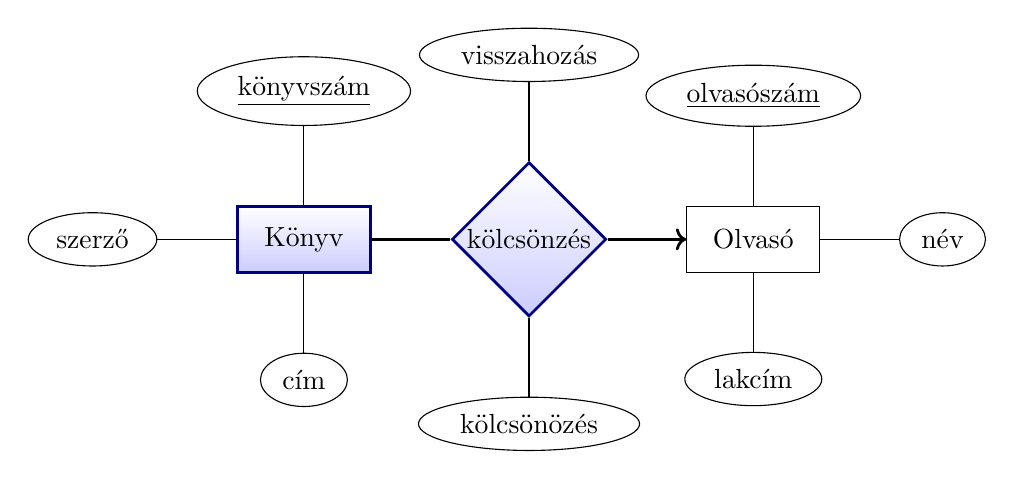
\begin{tikzpicture}[auto,node distance=1.0cm]
           \node[entity, top color=white, bottom color=blue!20, draw=blue!50!black!100,line width=1pt] (pgroup1) {Könyv};
           \node[attribute] (bnum) [above = of pgroup1] {\underline{könyvszám}} edge [-] (pgroup1);
           \node[attribute] (btitle) [below = of pgroup1] {cím} edge [-] (pgroup1);
           \node[attribute] (bauthor) [left = of pgroup1] {szerző} edge [-] (pgroup1);
           \node[relationship, top color=white, bottom color=blue!20, draw=blue!50!black!100,line width=1pt] (joins1) [right = of pgroup1] {kölcsönzés};
           \node[attribute] (in) [above = of joins1] {visszahozás} edge [-] (joins1);
           \node[attribute] (out) [below = of joins1] {kölcsönözés} edge [-] (joins1);
           \path[line width=1pt] (pgroup1) edge [-] (joins1);
           \node[entity] (pgroup2) [right = of joins1] {Olvasó};
           \node[attribute] (rname) [above = of pgroup2] {\underline{olvasószám}} edge [-] (pgroup2);
           \node[attribute] (rname) [right = of pgroup2] {név} edge [-] (pgroup2);
           \node[attribute] (raddress) [below = of pgroup2] {lakcím} edge [-] (pgroup2);
           \path[line width=1pt] (pgroup2) edge [<-] (joins1);
        \end{tikzpicture}
    \end{center}

    \begin{itemize}
      \item KÖNYV(\underline{könyvszám}, szerző, cím)
      \item OLVASÓ(\underline{olvasószám}, név, lakcím)
      \item KÖLCSÖNZÉS(könyvszám, olvasószám, kivétel, visszahozás)
    \end{itemize}

    \noindent \textit{Összetett attribútumok leképezése}: Például ha a lakcímet (helység, utca, házszám) struktúrában akarjuk kezelni, akkor fel kell venni a sémába mindet attribútumként.
    \begin{itemize}
      \item OLVASÓ(\underline{olvasószám}, név, helység, utca, házszám)
    \end{itemize}

	\noindent \textit{Többértékű attribútumok leképezése}:
	\begin{itemize}
        \item Megadás egyértékűként: \\
        Például egy több szerzős könyvnél egy mezőben soroljuk fel az összeset.\\
        Nem túl jó megoldás, mert nem lehet a szerzőket külön kezelni, és esetleg nem is fér el mind a mezőben.\\
        {\small
        KÖNYV(9635451903, Adatbázis rendszerek - Alapvetés, $\boldsymbol{\{}$\textbf{Jeffrey D. Ullman, Jennifer Widom}$\boldsymbol{\}}$)
        }
		\item Megadás többértékűként:
		\begin{itemize}
			\item \emph{Sorok többszörözése}: Felveszünk annyi sort, ahány szerző van. ($\Rightarrow$ redundancia)\\
            {\small
            KÖNYV(9635451903, Adatbázis rendszerek - Alapvetés, Jeffrey D. Ullman)\\
            KÖNYV(9635451903, Adatbázis rendszerek - Alapvetés, Jennifer Widom)
            }
        \item \emph{Új tábla hozzáadása}: A {\small KÖNYV(könyvszám, szerző, cím)} sémát az alábbi két sémával helyettesítjük:
        \begin{itemize}
            \small
            \item KÖNYV(\underline{könyvszám}, cím),
            \item SZERZŐ(\underline{könyvszám}, \underline{szerző})
        \end{itemize}
		\item \emph{Sorszámozás}: Ha nem mindegy a szerzők sorrendje, akkor az előző megoldásban (új tábla) ki kell egészíteni a szerző táblát egy sorszám mezővel.
        \begin{itemize}
            \small
            \item KÖNYV(\underline{könyvszám}, cím),
            \item SZERZŐ(\underline{könyvszám}, \textbf{sorszám}, \underline{szerző})
        \end{itemize}
		\end{itemize}
	\end{itemize}

	\subsection*{Kapcsolatok leképezése}
	\begin{itemize}
        \item \textbf{egy-egy}: Az egyik sémát (tetszőleges, hogy melyiket) bővítjük a másik kulcsával és a kapcsolat attribútumaival.\\

        Például: Ha egy olvasónak egyszerre csak egy könyvet adnak ki, akkor a kölcsönzés 1:1 kapcsolatot jelent. Ilyenkor a KÖLCSÖN sémában a könyvszám és az olvasószám egyaránt kulcs. Továbbá, a visszahozás attribútumra nincs szükségünk, mivel a könyv visszahozásával a könyv-olvasó kapcsolat megszűnik.\\

        Tehát, a
        \begin{itemize}
        \item {\small KÖLCSÖN (\underline{könyvszám}, olvasószám, kivétel)} vagy a
        \item {\small KÖLCSÖN (könyvszám, \underline{olvasószám}, kivétel)} sémát vehetjük fel a kapcsolathoz.\\
        \end{itemize}

        A KÖLCSÖN sémát az azonos kulcsú sémába olvasztva a
        {\small
        \begin{itemize}
            \item KÖNYV(\underline{könyvszám}, szerző, cím, \textbf{olvasószám, kivétel})
            \item OLVASÓ(\underline{olvasószám}, név, lakcím)
        \end{itemize}
        } vagy a
        {\small
        \begin{itemize}
            \item KÖNYV(\underline{könyvszám}, szerző, cím)
            \item OLVASÓ(\underline{olvasószám}, név, lakcím, \textbf{könyvszám, kivétel})
        \end{itemize}
        }
        adatbázissémákat kapjuk.
        \item \textbf{egy-sok}: az N oldali egyedhez tartozó sémát bővítjük az 1 oldali egyed kulcsával.\\

        Például: Ha egy olvasó több könyvet is kikölcsönözhet, akkor az olvasó-könyv kapcsolat 1:N típusú. Ekkor a KÖLCSÖN sémában csak a könyvszám lehet kulcs, ezért a KÖLCSÖN sémát csak a KÖNYV sémába olvaszthatjuk:
        {\small
        \begin{itemize}
            \item KÖNYV(\underline{könyvszám}, szerző, cím, olvasószám, kivétel)
            \item OLVASÓ(\underline{olvasószám}, név, lakcím)
        \end{itemize}
        }
        \item \textbf{sok-sok}: új sémát veszünk fel (benne: egyedek kulcsai, kapcsolat attribútumai).\\

        Például: Ha az egyes könyvek korábbi kölcsönzéseit is nyilvántartjuk, akkor nem csak egy olvasóhoz tartozhat több könyv, hanem egy könyvhöz is több olvasó (N:M kapcsolat), sőt adott olvasó adott könyvet egymás után többször is kikölcsönözhet.\\

        Ezért a KÖLCSÖN sémában {könyvszám, kivétel} vagy {könyvszám, visszahozás} a kulcs, a KÖLCSÖN táblát most sem a KÖNYV, sem az OLVASÓ táblába nem tudjuk beolvasztani.\\

        Az adatbázisséma ezért a következő:
        {\small
        \begin{itemize}
            \item KÖNYV(\underline{könyvszám}, szerző, cím)
            \item OLVASÓ(\underline{olvasószám}, név, lakcím)
            \item KÖLCSÖN(\underline{könyvszám}, olvasószám, kivétel, visszahozás)
        \end{itemize}
        }
	\end{itemize}
	
    \subsubsection*{Specializáló kapcsolatok átírása}


        \begin{center}
            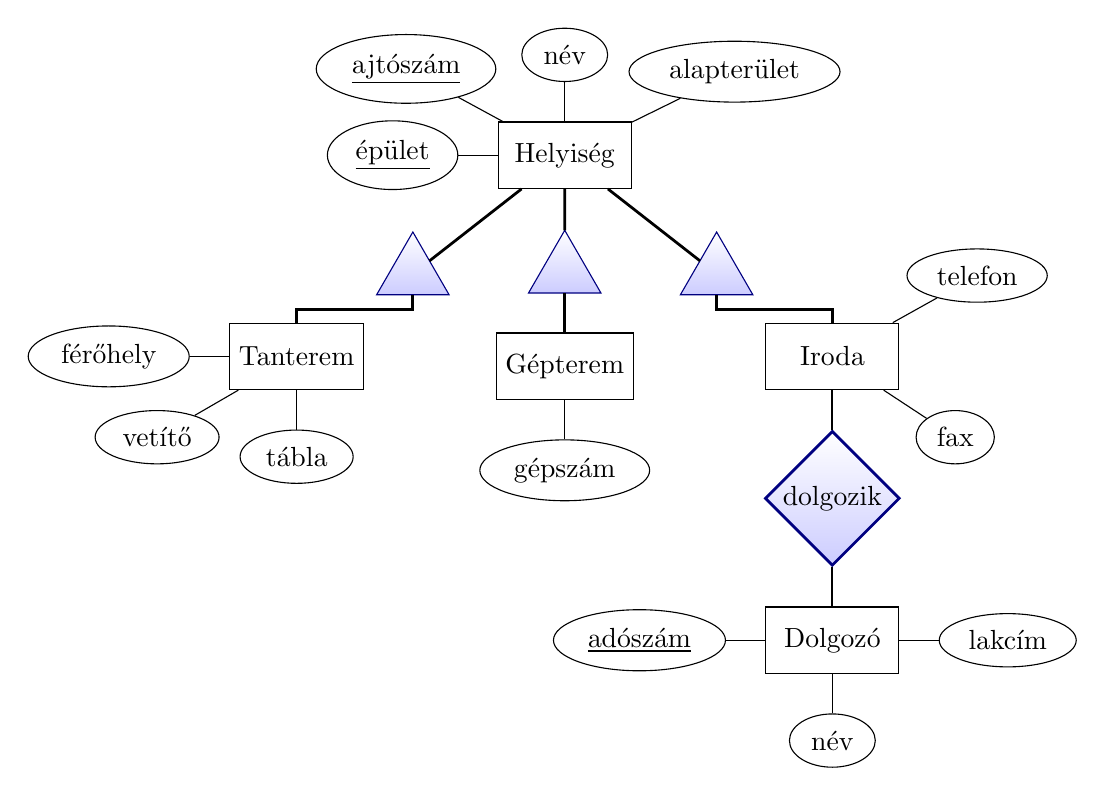
\begin{tikzpicture}[auto,node distance=1.25cm,
                amp/.style = {regular polygon, regular polygon sides=3,
                  draw, text width=0.5em,
                  inner sep=1mm, outer sep=0mm}]
                \node[entity] (node1) {Helyiség};
                \node[amp] (amp1) [node distance=1.25cm, below left = of node1,top color=white, bottom color=blue!20, draw=blue!50!black!100] {};
                \node[amp] (amp2) [node distance=0.525cm, below = of node1,top color=white, bottom color=blue!20, draw=blue!50!black!100] {};
                \node[amp] (amp3) [node distance=1.25cm, below right = of node1,top color=white, bottom color=blue!20, draw=blue!50!black!100] {};
                \node[attribute, node distance=0.5cm] (pattr1) [left = of node1] {\underline{épület}} edge [-] (node1);
                \node[attribute, node distance=0.5cm] (pattr2) [above left = of node1] {\underline{ajtószám}} edge [-] (node1);
                \node[attribute, node distance=0.5cm] (pattr3) [above = of node1] {név} edge [-] (node1);
                \node[attribute, node distance=0.5cm] (pattr4) [above right = of node1] {alapterület} edge [-] (node1);
                \path[line, line width=1pt] (node1) -- (amp1);
                \path[line, line width=1pt] (node1) -- (amp2);
                \path[line, line width=1pt] (node1) -- (amp3);
                \node[entity, node distance=0.5cm] (node2) [below left = of amp1] {Tanterem};
                \node[attribute, node distance=0.5cm] (pattr5) [left = of node2] {férőhely} edge [-] (node2);
                \node[attribute, node distance=0.5cm] (pattr6) [below left = of node2] {vetítő} edge [-] (node2);
                \node[attribute, node distance=0.5cm] (pattr7) [below = of node2] {tábla} edge [-] (node2);
                \node[entity, node distance=0.5cm] (node3) [below = of amp2, node distance=1.25cm] {Gépterem};
                \node[attribute, node distance=0.5cm] (pattr8) [below = of node3] {gépszám} edge [-] (node3);
                \node[entity, node distance=0.5cm] (node4) [below right = of amp3, node distance=1.25cm] {Iroda};
                \node[attribute, node distance=0.5cm] (pattr9) [above right = of node4] {telefon} edge [-] (node4);
                \node[attribute, node distance=0.5cm] (pattr10) [below right = of node4] {fax} edge [-] (node4);
                \node[relationship, node distance=0.5cm, top color=white, bottom color=blue!20, draw=blue!50!black!100,line width=1pt] (joins1) [below = of node4] {dolgozik};
                \path[line] (joins1) edge [-] (node4);
                \node[entity, node distance=0.5cm] (node5) [below = of joins1] {Dolgozó};
                \path[line] (joins1) edge [-] (node5);
                \node[attribute, node distance=0.5cm] (pattr11) [left = of node5] {\underline{adószám}} edge [-] (node5);
                \node[attribute, node distance=0.5cm] (pattr12) [below = of node5] {név} edge [-] (node5);
                \node[attribute, node distance=0.5cm] (pattr13) [right = of node5] {lakcím} edge [-] (node5);
                \path [line, line width=1pt] (amp1) -- ++(0pt,-13pt) -| (node2);
                \path [line, line width=1pt] (amp2) -- ++(0,-10pt) -| (node3);
                \path [line, line width=1pt] (amp3) -- ++(0pt,-13pt) -| (node4);
            \end{tikzpicture}
        \end{center}

	\paragraph*{Osztályhierarchia átírása\\}

	\begin{itemize}
        \item[(1)] Minden altípushoz külön tábla felvétele, egy egyed csak egy táblában szerepel. Az altípusok örökölik a főtípus attribútumait. \\

        (\emph{Objektumorientált stílusú reprezentálás})
        {\small
        \begin{itemize}
            \item HELYISÉG(\underline{épület}, \underline{ajtószám}, \emph{név, alapterület})
            \item TANTEREM(\underline{épület}, \underline{ajtószám}, \emph{név, alapterület}, férőhely, tábla, vetítő)
            \item GÉPTEREM(\underline{épület}, \underline{ajtószám}, \emph{név, alapterület}, gépszám)
            \item IRODA(\underline{épület}, \underline{ajtószám}, \emph{név, alapterület}, telefon, fax)
            \item DOLGOZÓ(\underline{adószám}, név, lakcím, épület, ajtószám)
        \end{itemize}
        }
        Hátrányai:
        \begin{itemize}
            \item Kereséskor gyakran több táblát kell vizsgálni (ha például a D épület 803. sz. terem alapterületét keressük).
            \item Kombinált altípus (például számítógépes tanterem) csak új altípus felvételével kezelhető.
        \end{itemize}
\newpage
        \item[(2)] Minden altípushoz külön tábla felvétele, egy egyed több táblában is szerepelhet. A főtípus táblájában minden egyed szerepel, és annyi altípuséban ahánynak megfelel. Az altípusok a főtípustól csak a kulcs-attribútumokat öröklik.\\

            (\emph{E/K stílusú reprezentálás})
        {\small
        \begin{itemize}
            \item HELYISÉG(\underline{épület}, \underline{ajtószám}, név, alapterület)
            \item TANTEREM(\underline{épület}, \underline{ajtószám}, férőhely, tábla, vetítő)
            \item GÉPTEREM(\underline{épület}, \underline{ajtószám}, gépszám)
            \item IRODA(\underline{épület}, \underline{ajtószám}, telefon, fax)
            \item DOLGOZÓ(\underline{adószám}, név, lakcím, épület, ajtószám)
        \end{itemize}
        }
        \emph{Hátrányai}:
        \begin{itemize}
            \item Előfordulhat, hogy több táblában kell keresni (például: ha a tantermek nevére és férőhelyére vagyunk kíváncsiak).
        \end{itemize}
        \item[(3)] Egy közös tábla felvétele, az attribútumok uniójával. Az aktuálisan értékkel nem rendelkező attribútumok NULL értékűek. \\

        (\emph{Reprezentálás nullértékekkel})
        {\small
        \begin{itemize}
            \item HELYISÉG(\underline{épület}, \underline{ajtószám}, név, alapterület, férőhely, tábla, vetítő, gépszám, telefon, fax)
            \item DOLGOZÓ(\underline{adószám}, név, lakcím, épület, ajtószám)
        \end{itemize}
        }
        \emph{Hátrányai}:
        \begin{itemize}
            \item Az ilyen egyesített táblában általában sok NULL attribútumérték szerepel.
            \item Elveszíthetjük a típusinformációt (például: ha a gépteremnél a gépszám nem ismert és ezért NULL, akkor a gépterem lényegében az egyéb helyiségek kategóriájába kerül).
        \end{itemize}
	\end{itemize}
\newpage
	\section*{Relációs algebra, SQL}
	
    \noindent \textit{Relációs algebra}: Az algebra szó a matematikában azt a diszciplínát jelöli, amely egy halmazon értelmezett műveletek tulajdonságait vizsgálja. A mi esetünkben a műveletek a relációkon értelmezettek, így innen származik a relációs algebra kifejezése. A műveletek tehát relációkon értelmezettek és ami nagyon fontos és lényeges, hogy relációkat is adnak eredményül. Tehát egy lekérdezés eredménye egy újabb relációt szolgáltat, vagyis a relációs algebrai műveletek nem vezetnek ki a relációk halmazából, a kapott eredmény szintén az adatbázis részének tekinthető.\\

	\subsection*{Relációs algebrai műveletek}
	
	\subsubsection*{Halmazműveletek}

    Legyen $R(A_1, \ldots, A_n)$ és $S(B_1, \ldots, B_m)$ tetszőleges relációséma és $n = m$, valamint
    \[
        dom(A_i) = dom(B_i) \qquad (\forall i)
    \]

    \noindent $R \bigcup S$ ($R$ és $S$ \emph{\textbf{uniója}}): $R \bigcup S = \textbf{F}(C_1, \ldots, C_n)$, ahol
    \[
        F := \Big\{f_i\ \Big|\ f_i \in R \vee f_i \in S\ \ \wedge\ \ (f_i \neq f_j \quad  \forall i, j \in n,\ i \neq j)\Big\}
    \]
    \begin{itemize}
        \item $R$, $S$ és \textbf{F} azonos sémájú.
        \item \textbf{F} nem tartalmaz azonos sorokat. (Ez gyakorlatban eltérhet)
        \item $\Big|R \bigcup S\Big| \leq \Big|R\Big| + \Big|S\Big|$
        \item Nem feltétlenül örököl típusneveket vagy attribútumneveket.
        \item \emph{SQL}: SELECT * FROM R \textbf{UNION} SELECT * FROM S;
    \end{itemize}

    \noindent \textit{Példa}:

    \begin{center}
        $R := \begin{array}{|c|c|}
         \hline
            \text{\textbf{A}} & \text{\textbf{B}} \\ \hline \hline
            0 & 0 \\ \hline
            0 & 1 \\ \hline
        \end{array} \qquad S := \begin{array}{|c|c|}
         \hline
            \text{\textbf{A}} & \text{\textbf{B}} \\ \hline \hline
            0 & 0 \\ \hline
            1 & 0 \\ \hline
        \end{array} \qquad
        R \bigcup S := \begin{array}{|c|c|}
         \hline
            \text{\textbf{A}} & \text{\textbf{B}} \\ \hline \hline
            0 & 0 \\ \hline
            0 & 1 \\ \hline
            1 & 0 \\ \hline
        \end{array}$
    \end{center}

    \noindent $R \setminus S$ ($R$ és $S$ \emph{\textbf{különbsége}}):  $R \setminus S = \textbf{F}(C_1, \ldots, C_n)$, ahol
    \[
        F := \Big\{f_i\ \Big|\ f_i \in R \wedge f_i \not \in S\Big\}
    \]
    \begin{itemize}
        \item $R$ azon sorait tartalmazza, amelyeket $S$ nem tartalmazza.
        \item $\Big|R \setminus S\Big| \leq \Big|R\Big|$
        \item Fontos: $R \setminus S \neq S \setminus R$ (nem kommutatív).
        \item Örökli a típusneveket és az attribútum neveket, mert $R \setminus S \subseteq R$.
        \item \emph{SQL}: SELECT * FROM R \textbf{MINUS} SELECT * FROM S;
    \end{itemize}

    \noindent \textit{Példa}:
    \begin{center}
        $R := \begin{array}{|c|c|}
         \hline
            \text{\textbf{A}} & \text{\textbf{B}} \\ \hline \hline
            0 & 0 \\ \hline
            0 & 1 \\ \hline
        \end{array} \qquad S := \begin{array}{|c|c|}
        \hline
            \text{\textbf{A}} & \text{\textbf{B}} \\ \hline \hline
            0 & 0 \\ \hline
            1 & 0 \\ \hline
        \end{array} \qquad
        R \setminus S := \begin{array}{|c|c|}
         \hline
            \text{\textbf{A}} & \text{\textbf{B}} \\ \hline \hline
            0 & 1 \\ \hline
        \end{array}$
    \end{center}

    \noindent $R \times S$ ($R$ és $S$ \emph{\textbf{Descartes-szorzata}}): Az $R$ és $S$ minden sora párban összefűződik, az első reláció minden sorához hozzáfűzzük a második reláció minden sorát.
    \begin{itemize}
        \item $R$ minden sorát tartalmazza $S$ minden sorával az összes kombinációban.
        \item $R \times S$ sémája $R$ és $S$ sémájának egyesítése.
        \item Ha R, S sémáiban nincs közös attribútum, akkor $R \bowtie S = R \times S$
        \item $\Big|R \times S\Big| = \Big|R\Big| * \Big|S\Big|$
        \item \emph{SQL}: SELECT * FROM R \textbf{CROSS JOIN} S vagy SELECT * FROM R\textbf{,} S;
    \end{itemize}

    \noindent \textit{Példa}:

    \begin{center}
        $R := \begin{array}{|c|c|}
            \hline
            \text{\textbf{A}} & \text{\textbf{B}} \\ \hline \hline
            0 & 0 \\ \hline
            0 & 1 \\ \hline
        \end{array} \qquad S := \begin{array}{|c|c|}
            \hline
            \text{\textbf{B}} & \text{\textbf{C}} \\ \hline \hline
            0 & 0 \\ \hline
            1 & 0 \\ \hline
        \end{array} \qquad
        R \times S := \begin{array}{|c|c|c|c|}
            \hline
            \text{\textbf{A}} & \text{\textbf{R.B}} & \text{\textbf{S.B}} & \text{\textbf{C}} \\ \hline \hline
            0 & 0 & 0 & 0 \\ \hline
            0 & 0 & 1 & 0 \\ \hline
            0 & 1 & 0 & 0 \\ \hline
            0 & 1 & 1 & 0 \\ \hline
        \end{array}$
    \end{center}

	\noindent Az alapműveletekhez az \emph{unió} és \emph{különbség} és a Descartes-szorzat tartozik.\\
    \noindent A \emph{metszet} műveletet származtatjuk:
    \begin{center}
        $R \bigcap S = R \setminus (R \setminus S)$
    \end{center}

    \noindent $R \bigcap S$ ($R$ és $S$ \emph{\textbf{metszete}}): $R \bigcap S = \textbf{F}(C_1, \ldots, C_n)$, ahol
    \[
        F := \Big\{f_i\ \Big|\ f_i \in R \wedge f_i \in S\ \ \wedge\ \ (f_i \neq f_j \quad  \forall i, j \in n,\ i \neq j)\Big\}
    \]
    \begin{itemize}
        \item $R$ azon sorait tartalmazza, amelyeket $S$ is tartalmazza.
        \item $R$, $S$ és \textbf{F} azonos sémájú.
        \item \textbf{F} nem tartalmaz azonos sorokat.
        \item $\big|R \cap S\big| = \big|R\big| + \big|S\big|$
        \item \emph{SQL}: SELECT * FROM R \textbf{INTERSECT} SELECT * FROM S;
    \end{itemize}

    \noindent \textit{Példa}:
    \begin{center}
        $R := \begin{array}{|c|c|}
             \hline
                \text{\textbf{A}} & \text{\textbf{B}} \\ \hline \hline
                0 & 0 \\ \hline
                0 & 1 \\ \hline
            \end{array} \qquad S := \begin{array}{|c|c|}
            \hline
                \text{\textbf{A}} & \text{\textbf{B}} \\ \hline \hline
                0 & 0 \\ \hline
                1 & 0 \\ \hline
            \end{array} \qquad
            R \bigcap S := \begin{array}{|c|c|}
             \hline
                \text{\textbf{A}} & \text{\textbf{B}} \\ \hline \hline
                0 & 0 \\ \hline
        \end{array}$
    \end{center}

	\paragraph*{Vetítés (projekció)}

    $\boldsymbol{\Pi}_{A_{i_1}, \ldots, A_{i_k}}(R)$ ($R$ \emph{\textbf{vetítése}}): $R$ relációból olyan új relációt hoz létre, amelyik csak $R$ bizonyos attribútumait tartalmazza:
    \[
        \Pi_{A_{i_1}, \ldots, A_{i_k}}(R) := \Big\{t.A_{i_1}, t.A_{i_2},\ \ldots,\ t.A_{i_k} \big|\ t \in R \Big\}
    \]
    \begin{itemize}
        \item Számít az attribútumok sorrendje. (rendezett lista)
        \item $\Big|\Pi_{A_{i_1}, \ldots, A_{i_k}}(R)\Big| < \Big|R\Big|$
        \item Örökli a típusneveket és az attribútum neveket.
   \end{itemize}

   \noindent \textit{Példa:}

    $R := \begin{array}{|c|l|c|}
        \hline
        \text{ID} & \text{Név} & \text{Kor} \\ \hline \hline
        1 & \text{Péter} & 3  \\ \hline
        2 & \text{László} & 37 \\ \hline
    \end{array} \qquad \Pi_{\text{ID}, \text{Név}}(R) :=
    \begin{array}{|c|l|}
        \hline
        \text{ID} & \text{Név} \\ \hline \hline
        1 & \text{Péter}  \\ \hline
        2 & \text{László} \\ \hline
    \end{array}
    $

    \  \\

    \paragraph*{Kiválasztás (szelekció)}

    $\boldsymbol{\sigma}_{C}(R)$ ($R$ \emph{\textbf{szelekciója}}): $R$ reláció azon sorai, amelyekre az $C$ feltétel igaz.

    \begin{itemize}
        \item $C$ feltétel lehet:
        \begin{itemize}
            \item \emph{Elemi}: $A_i\ \theta\ A_j$, $A_i\ \theta\ d$, ahol $d$ konstans, $\theta \in \Big\{=, <, >, \neq, \leq, \geq\Big\}$.
            \item \emph{Összetett}: ha $B_1, B_2$ feltétel, akkor $\neg B_1, B_1 \bigcap B_2, B_1 \bigcup B_2$ és a zárójelezések is feltétel.
        \end{itemize}
        \item C feltétel \emph{\textbf{nem tartalmazhat függvényeket}}: $C = A + B < 5$
        {\small
        \item Összetett feltételek átírhatók elemi feltételeket használó kifejezésekké
        \begin{itemize}
            \item $\sigma_{F_1 \wedge F_2}(R) \cong \sigma_{F_1}(\sigma_{F_2}(R)) \cong \sigma_{F_2}(\sigma_{F_1}(R))$
            \item $\sigma_{F_1 \vee F_2}(R) \cong \sigma_{F_1}(R) \bigcup \sigma_{F_2}(R)$
            \item $\neg (F_{1} \wedge F_{2}) \Rightarrow (\neg F_{1}) \vee (\neg F_{2})$
            \item $\neg (F_{1} \vee F_{2}) \Rightarrow (\neg F_{1}) \wedge (\neg F_{2})$
            \item $\neg (A < B) \Rightarrow(A \geq B)$
        \end{itemize}
        }
        \item Örökli a típusneveket és az attribútum neveket, mivel $\sigma_{C}(R) \subseteq R$.
        \item $\Big|\sigma_{C}(R)\Big| < \Big|R\Big|$
        \item \emph{SQL}: SELECT * FROM R \textbf{WHERE $<$FELTÉTEL$>$};\\
    \end{itemize}

   \noindent \textit{Példa:}

    \begin{center}
        $R := \begin{array}{|c|l|c|}
            \hline
            \text{ID} & \text{Név} & \text{Kor} \\ \hline \hline
            1 & \text{Péter} & 3  \\ \hline
            2 & \text{László} & 37 \\ \hline
        \end{array} \qquad \sigma_{\text{Kor} > 10}(R) :=
        \begin{array}{|c|l|c|}
            \hline
            \text{ID} & \text{Név} & \text{Kor} \\ \hline \hline
            2 & \text{László} & 37 \\\hline
        \end{array}$
    \end{center}

    \ \\

    \paragraph*{Természetes összekapcsolás}

    Szorzás jellegű műveletek közül csak ez alapművelet. Nő az attribútumok száma. A közös attribútumnevekre épül: $R \bowtie S$ azon sorpárokat tartalmazza R-ből illetve S-ből, amelyek R és S azonos attribútumain megegyeznek. $R \bowtie S$ típusa a két attribútumhalmaz uniója.
    \begin{itemize}
        \item Ha R, S sémái megegyeznek, akkor $R \bowtie S = R \bigcap S$
        \item \emph{SQL}:
        \begin{itemize}
            \item SELECT * FROM R NATURAL JOIN S vagy
            \item SELECT DISTINCT A, R.B, C FROM R\textbf{,} S WHERE R.B = S.B;
        \end{itemize}
    \end{itemize}

    \noindent \textit{Példa}:

    \begin{center}
        $R := \begin{array}{|c|c|}
            \hline
            \textbf{A} & \textbf{B} \\ \hline \hline
            a & a \\ \hline
            c & b \\ \hline
            b & c \\ \hline
        \end{array} \qquad S := \begin{array}{|c|c|}
            \hline
            \textbf{B} & \textbf{C} \\ \hline \hline
            a & a \\ \hline
            a & c \\ \hline
            b & d \\ \hline
            e & d \\ \hline
        \end{array} \qquad R \bowtie S := \begin{array}{|c|c|c|}
            \hline
            \textbf{A} & \textbf{R.B} & \textbf{C} \\ \hline \hline
            a & a & a \\ \hline
            a & a  & c \\ \hline
            c & b & d \\ \hline
        \end{array}$
    \end{center}

    \noindent Szorzásjellegű műveletnél tekinthetjük a \textit{direkt-szorzatot} alapműveletnek, de a természetes összekapcsolást használják. A direkt-szorzat (vagy szorzat, Descartes-szorzat) esetén természetesen nem fontos az attribútumok egyenlősége. A két vagy több reláció azonos nevű attribútumait azonban meg kell különböztetni egymástól (átnevezéssel). \\

	\paragraph*{Átnevezés}

    $\rho_{B(D_{1}, \ldots, D_{k})}(R)$ ($R$ \emph{\textbf{átnevezése}}): $R$ reláció sémájának átnevezése $B$-re, valamint $R$ attribútumainak átnevezése $A_1, \ldots, A_n$-ről $D_{1}, \ldots, D_{n}$-re.
    \begin{itemize}
        \item $\rho_{B(D_1, \ldots, D_n)}(R)$ sémája $B(D_1, \ldots, D_n)$
        \item $\Big|\rho_{B(D_1, \ldots, D_n)}(R)\Big| = \Big|R\Big|$
        \item SQL:
        \begin{itemize}
            \item SELECT A, B, C \textbf{D} FROM R \textbf{B} vagy
            \item SELECT A, B, C \textbf{AS D} FROM R \textbf{AS B};\\
         \end{itemize}
    \end{itemize}

    \noindent \textit{Példa}:

    \begin{center}
        $R := \begin{array}{|c|c|c|}
            \hline
            \text{ID} & \text{Név} & \text{Fizetés} \\ \hline \hline
            1 & \text{Péter} & 300000  \\ \hline
            2 & \text{László} & 507000 \\ \hline
        \end{array} \qquad \rho_{B(\text{ID}, \text{Név}, \text{Jövedelem})}(R) :=
        \begin{array}{|c|c|c|}
            \hline
            \text{ID} & \text{Név} & \text{Jövedelem} \\ \hline \hline
            1 & \text{Péter} & 300000  \\ \hline
            2 & \text{László} & 507000 \\ \hline
        \end{array} := B$ \\
    \end{center}

    \ \\

    \noindent A relációs algebrában a $\bigcup, \setminus, \times (\bowtie), \Pi, \sigma, \rho$ alapműveletek találhatóak. Ez egy \textit{minimális készlet}, vagyis bármelyiket elhagyva az a többivel nem fejezhető ki. A kivonás egy kivétel, mert nem fejezhető ki a többi alapművelettel.\\

    \noindent $R \div S$ \textit{(\textbf{osztás})}: maradékos osztás mintájára. R és S sémája $R(A_1,...,A_n,B_1,...,B_m)$, illetve $S(B_1,...,B_m)$, $Q = R \div S$ sémája $Q(A_1,...,A_n)$. $R \div S$ a legnagyobb (legtöbb sort tartalmazó) reláció, amelyre $( R \div S ) \times S \subseteq R.$\\

    \noindent Relációs algebrában: $R(A,B) \div S(B) = \Pi_{A_1, \ldots, A_n}(R) – \Pi_{A_1,...,A_n}( \Pi_{A_1, \ldots, A_n}(R) \times S \setminus R )$\\

    \noindent \textit{Példa}:

    \begin{center}
        $R := \begin{array}{|c|c|}
            \hline
            \textbf{A} & \textbf{B} \\ \hline \hline
            F & A \\ \hline
            F & B \\ \hline
            F & C \\ \hline
            M & A \\ \hline
            M & B \\ \hline
            K & A \\ \hline
            K & D \\ \hline
            N & E \\ \hline
        \end{array} \qquad S := \begin{array}{|c|}
            \hline
            \textbf{B} \\ \hline \hline
            A \\ \hline
            B \\ \hline
        \end{array} \qquad R \div S := \begin{array}{|c|}
            \hline
            \textbf{A} \\ \hline \hline
            F \\ \hline
            M \\ \hline
        \end{array}$
    \end{center}

	\subsection*{Relációs algebra kiterjesztése\\}
	
    \noindent A relációkra vonatkozó műveleteket kiterjesztjük halmazokról multihalmazokra (sorok ismétlődése megengedett).\\
\newpage
	\noindent $\boldsymbol{\delta}(R)$ (\textbf{\emph{ismétlődések megszüntetése}}): Multihalmazból halmazt csinál.
        \begin{itemize}
            \item Örökli a típusneveket és az attribútum neveket, mivel $\delta(R) \subseteq R$.
            \item $\Big|\delta(R)\Big| \leq \Big|R\Big|$
            \item SQL: SELECT \textbf{DISTINCT} * FROM R;
        \end{itemize}

    \noindent \textit{Példa}:

        \begin{center}
            $R := \begin{array}{|c|c|}
                \hline
                \text{Név} & \text{Jövedelem} \\ \hline \hline
                \text{Péter} & 300000  \\ \hline
                \text{László} & 507000 \\ \hline
                \text{László} & 507000 \\ \hline
            \end{array} \qquad \delta(R) :=
            \begin{array}{|c|c|}
                \hline
                \text{Név} & \text{Jövedelem} \\ \hline \hline
                \text{Péter} & 300000  \\ \hline
                \text{László} & 507000 \\ \hline
            \end{array}$
    \end{center}

		\noindent $\boldsymbol{\Pi}_{L}(R)$ (\textbf{\emph{vetítési művelet kiterjesztése}}): A normál vetítési művelet kiterjesztett változata.\\

        \noindent A $L$ tartalmazhatja:
		\begin{itemize}
			\item R egy attribútumát,
			\item E $\to$ z, ahol E az R reláció attribútumaira vonatkozó (konstansokat, aritmetikai műveleteket, függvényeket tartalmazó kifejezés), z pedig az E kifejezés által számolt az eredményekhez tartozó új attribútum nevét jelöli. \\
		\end{itemize}

    \noindent \textit{Példa}:

        \begin{center}
            $R := \begin{array}{|c|c|}
                \hline
                \text{A} & \text{B} \\ \hline \hline
                1 & 2  \\ \hline
                2 & 3 \\ \hline
                4 & 5 \\ \hline
            \end{array} \qquad \Pi_{A+B \to C}(R) :=
            \begin{array}{|c|}
                \hline
                C \\ \hline \hline
                3  \\ \hline
                5 \\ \hline
                9 \\ \hline
            \end{array}$
        \end{center}

        \noindent $\boldsymbol{\gamma}_{L}(R)$ (\textbf{\emph{Összesítő műveletek és csoportosítás}}): A csoportosítást, a csoportokon végezhető összesítő függvényeket (AVG, SUM, COUNT, MIN. MAX, stb.) reprezentálja a művelet.
        \noindent Itt az $L$ valamennyi eleme a következők egyike:
		\begin{itemize}
			\item R olyan attribútuma, amely szerepel a GROUP BY záradékban, egyike a csoportosító attribútumoknak.
			\item R egyik attribútumára alkalmazott összesítő operátor.
            \begin{itemize}
                \item Ha az összesítés eredményére névvel szeretnénk hivatkozni, akkor nyilat és új nevet használunk.
            \end{itemize}
		\end{itemize}
        \noindent Értelmezése, kiértékelés: R sorait csoportokba osztjuk. Egy csoport azokat a sorokat tartalmazza, amelyek a listán szereplő csoportosítási attribútumokhoz tartozó értékei megegyeznek.
        \begin{itemize}
            \item Vagyis ezen attribútumok minden egyes különböző értéke egy csoportot alkot.
        \end{itemize}
        Minden egyes csoporthoz számoljuk ki a lista összesítési attribútumaira vonatkozó összesítéseket. Az eredmény minden egyes csoportra egy sor:
		\begin{enumerate}
			\item a csoportosítási attribútumok és
			\item az összesítési attribútumra vonatkozó összesítése	(az adott csoport összes sorára)
		\end{enumerate}

    \noindent $\boldsymbol{\tau}_{A_, \ldots, A_n}(R)$ (\textbf{\emph{rendezés}}): Először $A_1$ attribútum szerint rendezzük R sorait. Majd azokat a sorokat, amelyek értéke megegyezik az $A_1$ attribútumon, $A_2$ szerint, és így tovább. \\
	Ez az egyetlen olyan művelet, amelynek az eredménye se nem halmaz, se nem multihalmaz, hanem egy rendezett lista.
    \begin{itemize}
        \item $\tau(R)| = \Big|R\Big|$
        \item \emph{SQL}: SELECT A, B FROM R \textbf{ORDER BY} B;\\
    \end{itemize}

    \noindent \textit{Példa}:

    \begin{center}
        $R := \begin{array}{|c|c|}
                \hline
                \textbf{A} & \textbf{B} \\ \hline \hline
                1 & 2  \\ \hline
                3 & 4 \\ \hline
                5 & 2 \\ \hline
            \end{array} \qquad \tau(R) :=
            \begin{array}{|c|c|}
                \hline
                \textbf{A} & \textbf{B} \\ \hline \hline
                1 & 2  \\ \hline
                5 & 2 \\ \hline
                3 & 4 \\ \hline
        \end{array}$
    \end{center}

    \ \\

	\paragraph*{Algebrai kifejezés kiértékelése\\}

    \noindent Összetett kifejezést kívülről befelé haladva átírjuk kiértékelő fává, ahol a levelek elemi kifejezések.\\

    \noindent Legyen $R, S$ az $R(A, B, C), S(C, D, E)$ séma feletti reláció
    \[
        \Pi_{B,D}\sigma_{A = 'c' \wedge E = 2}(R \bowtie S)
    \]

    \noindent A kifejezéshez tartozó kifejezésfa (kiértékelése alulról felfelé történik)

    \begin{center}
        \begin{tikzpicture}
            \tikzstyle{level 1}=[sibling distance=10mm]
            \tikzstyle{level 2}=[sibling distance=10mm]
            \tikzstyle{level 3}=[sibling distance=30mm]

             \node{$\Pi_{B,D}$}
               child
               {
                node
                {
                    $\sigma_{A = 'c' \wedge E = 2}$
                }
                child
                    {
                        node {$\bowtie$}
                        child { node { R }}
                        child { node { S }}
                    }
               };
        \end{tikzpicture}
    \end{center}

	\subsection*{SQL\\}

    \noindent Az SQL kifejezés a Structured Query Language rövidítése, ami strukturált lekérdező nyelvet jelent. A relációs adatbázis-kezelő rendszerekben tárolt adatok kezelésére fejlesztették ki.\\\
\newpage	
    \noindent Az SQL széles körben népszerű, mert a következő előnyöket kínálja.
    Lehetővé teszi a felhasználók számára:
    \begin{itemize}
        \item az adatok leírását.
        \item a relációs adatbázis-kezelő rendszerek adatainak elérését.
        \item adatbázisokat és táblázatokat hozzanak létre vagy dobjanak el.
        \item az adatbázisban lévő adatok definiálását és az adatok manipulálását.
        \item nézetek létrehozását egy adatbázisban.
        \item táblák, eljárások és nézetek engedélyeinek beállítását.
    \end{itemize}

    \noindent Lehetővé teszi más nyelveken belüli beágyazást SQL modulok, könyvtárak és előfordítók használatával.\\

    \noindent Az első verzió alapjait az IBM fektette le a 70-es években. A nyelv elvi alapjait a relációs adatmodell fogalma, az Edgar F. Codd által leírt 12 szabálya adta. 80-as években az ANSI és ISO is szabványként fogadta el az SQL nyelvet.\\

    \noindent Az SQL nyelvi elemeket négyféleképp csoportosíthatjuk:
    \begin{itemize}
        \item \textbf{\emph{Adatdefiníciós, DDL}} (Data Definition Language)
        \item \textbf{\emph{Adatmanipulációs, DML}} (Data Manipulation Language)
        \item \textbf{\emph{Adatvezérlő, DCL}} (Data Control Language)
        \item \textbf{\emph{Lekérdező, DQL}} (Data Query Language)\\
    \end{itemize}

    \noindent Alap tulajdonságok:
    \begin{itemize}
        \item A nyelvben az egyes utasításokat pontosvessző válassza el egymástól.
        \item Az SQL case insensitive, tehát a kis és nagy betűk nincsenek megkülönböztetve egymástól.
        \item A parancsok tetszőlegesen tagolhatók (szóköz, tabulátor) és több sorba írhatók.
        \item A szöveg konstansokat szimpla aposztrófok jelölik pl.: 'SQL'
    \end{itemize}

    \ \\

	\noindent \emph{SQL-ben a relációt táblának nevezik}, amiből alapvetően három féle létezik:
    \begin{itemize}
        \item TABLE (alaptábla, permanens),
        \item VIEW (nézettábla),
        \item WITH utasítással (átmeneti munkatábla).
    \end{itemize}

	\subsubsection*{DDL (Data Definition Language)}

   \noindent Adatleíró rész az adatbázis objektumainak a leírására és megváltoztatására.

	\begin{itemize}
		\item CREATE: Adatbázis-objektum létrehozása.
{\small
        \begin{verbatim}
    CREATE DATABASE Nyilvantartas;

    CREATE TABLE alkalmazottak(
        id INT(11) NOT NULL,
        nev VARCHAR(70) NOT NULL,
        szuletesi_datum DATE  NOT NULL,
        irsz NUMBER(7) NOT NULL,
        varos VARCHAR(40) NOT NULL,
        cim VARCHAR(60) NOT NULL
    );

    CREATE VIEW alk_varosok AS
        SELECT id, nev, varos
        FROM alkalmazottak;
        \end{verbatim}
}
	   \item ALTER: Adatbázis-objektum módosítása.
        \begin{verbatim}
    ALTER TABLE alkalmazottak ADD cim VARCHAR(80);
        \end{verbatim}
	   \item DROP: Adatbázis-objektum megszüntetése. Minden, ami ehhez az elemhez kapcsolódott, elérhetetlen lesz.
        \begin{verbatim}
    DROP TABLE alkalmazottak;
    DROP VIEW alk_varosok;
        \end{verbatim}
        \item TRUNCATE TABLE: Tábla összes sorának törlése a tábla szerkezetének megtartásával.
	\end{itemize}

    \paragraph*{Megszorítások\\}

    \noindent A \textit{megszorítás} adatelemek közötti kapcsolat, amelyet az adatbázis-rendszernek fent kell tartania. Lehet kulcs megszorítás, értékekre, sorokra vonatkozó. Itt alapvetően az adatbázis bármely módosítása előtt ellenőrizni kell. Egy okos rendszer felismeri, hogy mely változtatások, mely megszorításokat érinthetnek. \\

    \noindent Megszorítás megadása CONSTRAINTS kulcsszóval történik. Saját megszorítás megadása: CREATE ASSERTION $<$név$>$ CHECK ($<$feltétel$>$).

    \begin{itemize}
        \item UNIQUE: Az adott oszlopban minden érték egyedi. Hatására index állomány jön létre. Felvehet NULL értéket.
        {\small
        \begin{verbatim}
CREATE TABLE Persons (
    ...
    CONSTRAINT UC_Person UNIQUE (ID,LastName)
);
        \end{verbatim}
        }
            \item PRIMARY KEY: Az adott oszlop a tábla elsődleges kulcsa lesz, megköveteli az adott oszlopban az értékek egyediségét. Oszlop-megszorításokban csak akkor tudunk elsődleges kulcsot definiálni, ha az elsődleges kulcs csak egy oszlopból áll. Ilyen oszlop csak egy lehet a táblában. Hatására mindig létrejön egy index állomány. Nem lehet NULL az értéke.
            {\small
            \begin{verbatim}
CREATE TABLE Persons (
    ...
    CONSTRAINT PK_Person PRIMARY KEY (ID,LastName)
);
            \end{verbatim}
            }
            \item FOREIGN KEY - Idegen kulcs egy másik tábla megfelelő oszlopára.
            \begin{itemize}
                \item REFERENCES kapcsolttabla(kapcsoltoszlop) [ON-feltételek]: Az adott oszlop idegen kulcs-hivatkozást tartalmaz a \emph{kapcsolttabla} \emph{kapcsoltoszlop}ára. A \emph{kapcsolttabla} \emph{kapcsoltoszlop}a csak elsődleges, vagy egyedi kulcs lehet.
            \end{itemize}
            Idegen kulcs (R-ről S-re) megszorítást meg kell őrizni, ez kétféleképpen sérülhet:
            \begin{enumerate}
                \item Egy R-be történő beszúrásnál vagy R-ben történő módosításnál S-ben nem szereplő értéket adunk meg.
                \item Egy S-beli törlés vagy módosítás ,,lógó" sorokat eredményez R-ben. Védeni többféleképpen lehet: alapértelmezetten nem hajtja végre, tovább gyűrűzésnél igazítjuk a tábla értékeit a változáshoz, SET NULL-nál pedig az érintett sorokat NULL-ra állítjuk.
            \end{enumerate}
            {\small
            \begin{verbatim}
CREATE TABLE Orders (
    ...
    CONSTRAINT FK_PersonOrder FOREIGN KEY (PersonID)
        REFERENCES Persons(PersonID)
);
            \end{verbatim}
            }
        \item DEFAULT: Alapértelmezett érték, mely akkor kerül az új sor adott oszlopába, ha nem adunk meg a beszúrás során implicit értéket.
            {\small
            \begin{verbatim}
CREATE TABLE Orders (
    ...
    OrderDate date DEFAULT GETDATE()
);
            \end{verbatim}
            }
        \item CHECK: Az oszlopra vonatkozó logikai kifejezést adhatunk meg, a feltételben csak az oszlop szerepelhet. A beszúrás, módosítás csak akkor történik meg, ha a kifejezés értéke igaz lesz.
        {\small
        \begin{verbatim}
CREATE TABLE Persons (
    ...
    Age int,
    CONSTRAINT CHK_Person CHECK (Age>=18)
);
        \end{verbatim}
        }
        \item NOT NULL | NULL: Az adott oszlopban szerepelhet-e NULL érték.
        {\small
        \begin{verbatim}
CREATE TABLE Persons (
    ...
    LastName varchar(255) NOT NULL,
    FirstName varchar(255) NOT NULL,
    ...
);
        \end{verbatim}
        }
    \end{itemize}

	\subsubsection*{DQL (Data Query Language)}

	\noindent Relációs algebrai kifejezések felírása SELECT-tel:
	\begin{itemize}
		\item SELECT lista FROM táblák szorzata WHERE felt. = $\Pi_{lista}\big(\sigma_{felt.}$(táblák szorzata)\big)
		\item Halmazműveletek: \textbf{UNION}, \textbf{EXCEPT}/\textbf{MINUS}, \textbf{INTERSECT}. Multihalmazból halmaz lesz. ALL kulcsszóval megmarad a multihalmaz.
		\item Átnevezés: oszlopnév után szóközzel odaírjuk az új nevet vagy AS új név.
	\end{itemize}

	\noindent Kiterjesztett műveletek:
	\begin{itemize}
		\item Rendezés: \textbf{ORDER BY}, minden más záradék után következik, csökkenő, növekvő sorrend.
		\item Ismétlődések megszüntetése: SELECT \textbf{DISTINCT} ...
        \item Összesítések (aggregálás): \textbf{SUM}, \textbf{COUNT}, \textbf{MIN}, \textbf{MAX}, \textbf{AVG} a SELECT záradékban. \textbf{COUNT}(*) az eredmény sorainak száma. Ha összesítés is szerepel a lekérdezésben, a SELECT-ben felsorolt attribútumok vagy egy összesítő függvény paramétereként szerepelnek, vagy a \emph{GROUP BY} attribútumlistájában is megjelennek.
		\item Csoportosítás: \textbf{GROUP BY}.
        \item Csoportok szűrése: \textbf{HAVING}. Csoportokat szűr, nem egy-egy sort. Az alkérdésre nincs megszorítás. Viszont az alkérdésen kívül csak olyan attribútumok szerepelhetnek, amelyek: vagy csoportosító attribútumok, vagy összesített attribútumok. (Azaz ugyanazok a szabályok érvényesek, mint a SELECT záradéknál).
	\end{itemize}
    {\small
    \begin{verbatim}
    SELECT név, AVG(jegy) AS átlag
    FROM hallgató
    GROUP BY azon, név
    HAVING COUNT(tantárgy) > 2;
    \end{verbatim}
    }

    \begin{center}
        \begin{tikzpicture}
            \tikzstyle{level 1}=[sibling distance=10mm]
            \tikzstyle{level 2}=[sibling distance=10mm]
            \tikzstyle{level 3}=[sibling distance=30mm]

             \node{$\Pi_{\text{név},\text{átlag}}$}
               child
               {
                node
                {
                    $\sigma_{db > 2}$
                }
                child
                    {
                        node {$\gamma_{\text{azon}, \text{név}, AVG(jegy) \to \text{átlag},\ COUNT(\text{tantárgy}) \to db}$}
                        child { node { \text{hallgató} }}
                    }
               };
        \end{tikzpicture}
    \end{center}

	\noindent WHERE záradéknál SQL-es specialitások
	\begin{itemize}
		\item Átírható relációs algebrába: \textbf{BETWEEN} ... \textbf{AND} ..., \textbf{IN}(értékhalmaz)
		\item Nem írható át relációs algebrába: \textbf{LIKE} karakterláncok összehasonlításánál, \textbf{IS NULL} (ismeretlen vagy nem definiált érték) [emiatt 3-értékű logika SQL-ben: true, false, unknown]
	\end{itemize}
\newpage
	\noindent SELECT utasítás több részből áll, a részeket záradékoknak nevezzük.\\

    \noindent Három alapvető záradék van:
	\begin{itemize}
		\item SELECT lista (3.) -- milyen típusú sort szeretnénk az eredményben látni? * jelentése: minden attribútum.
		\item FROM Relációnév (1.) -- a tábla neve vagy relációk (táblák) összekapcsolása, illetve szorzata
		\item WHERE feltétel (2.) -- milyen feltételeknek eleget tevő sorokat kiválasztani?
	\end{itemize}
	
\noindent Több séma összekapcsolása esetén, ha egy attribútumnév több sémában is előfordul, akkor kell hozzá a séma is a hivatkozásnál: R.A (R reláció A attribútuma). \\

	\noindent \textit{Alkérdéseket} is használhatunk SQL-ben. Ekkor az alkérdést zárójelbe tesszük.

	\begin{itemize}
		\item FROM záradékban ilyen módon ideiglenes táblát is létrehozhatunk, ekkor többnyire a sorváltozó nevét is meg kell adni hozzá.
		\item WHERE záradékban az alkérdés eredménye lehet:
		\begin{itemize}
			\item egy skalárérték, vagyis mintha egy konstans lenne
			\item skalár értékekből álló multihalmaz, logikai kifejezésekben használható: EXISTS, [NOT] IN, ANY/ALL (pl x $>$ ANY (alkérdés)).
			\item teljes többdimenziós tábla, használható: EXISTS, [NOT] IN
		\end{itemize}
	\end{itemize}

    \noindent Az alkérdés nem korrelált, ha önállóan kiértékelhető, külső kérdés közben nem változik. Korrelált, ha többször kerül kiértékelésre, alkérdésen kívüli sorváltozóból származó értékadással.\\

    \noindent Teljes SELECT utasítás (záradékok sorrendje nem cserélhető fel)
    \begin{verbatim}
    SELECT [DISTINCT] ...
    FROM ...
    [WHERE ...]
    [GROUP BY ...
        [HAVING ...]]
    [ORDER BY ...]
    \end{verbatim}

	\paragraph*{Összekapcsolások\\}

%      $\begin{tabular}{lc}
%        \makecell{\text{Descartes-szorzat}\\ \text{R CROSS JOIN S, vagy ,,R,S"}} & 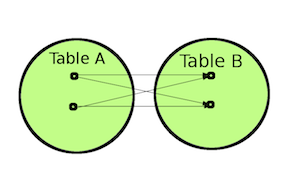
\includegraphics[width=0.35\linewidth]{img/cross-join.png} \\ \hline
%        \makecell{\text{Természetes összekapcsolás}\\ \text{R NATURAL JOIN S}} &  \\ \hline
%        \makecell{\text{Théta összekapcsolás}\\ \text{R INNER JOIN S ON $<$feltétel$>$}} & 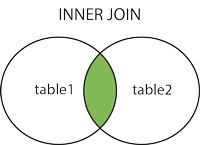
\includegraphics[width=0.25\linewidth]{img/img_innerjoin.jpg} \\ \hline
%        \makecell{\text{Külső összekapcsolás} \\ \text{R \{LEFT | RIGHT | FULL\} OUTER JOIN S}} & \makecell
%        {
%            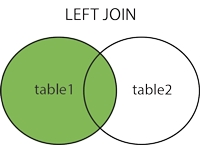
\includegraphics[width=0.25\linewidth]{img/img_leftjoin.jpg}\\
%            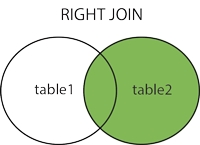
\includegraphics[width=0.25\linewidth]{img/img_rightjoin.jpg}\\
%            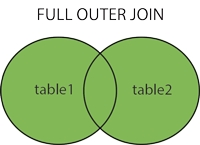
\includegraphics[width=0.25\linewidth]{img/img_fulljoin.jpg}
%        }  \\
%      \end{tabular}$

	\begin{itemize}
		\item Descartes-szorzat: R CROSS JOIN S, vagy ,,R,S"
%        \begin{center}
%            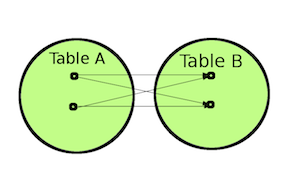
\includegraphics[width=0.35\linewidth]{img/cross-join.png}
%        \end{center}
		\item Természetes összekapcsolás: R NATURAL JOIN S
		\item Théta-összekapcsolás: R INNER JOIN S ON $<$feltétel$>$
%        \begin{center}
%            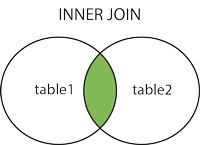
\includegraphics[width=0.25\linewidth]{img/img_innerjoin.jpg}
%        \end{center}
		\item Külső összekapcsolás: R $\{$LEFT $|$ RIGHT $|$ FULL$\}$ OUTER JOIN S. LEFT az R lógó sorait őrzi meg, RIGHT az S-ét, FULL az összeset.\\
%        \begin{center}
%            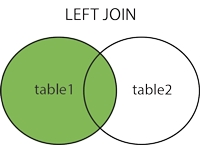
\includegraphics[width=0.25\linewidth]{img/img_leftjoin.jpg}
%            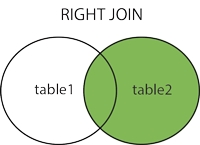
\includegraphics[width=0.25\linewidth]{img/img_rightjoin.jpg}
%            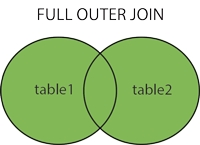
\includegraphics[width=0.25\linewidth]{img/img_fulljoin.jpg}
%        \end{center}
	\end{itemize}

    \subsection*{DCL (Data Control Language)}

    \noindent GRANT - a felhasználó hozzáférési jogosultságokat ad az adatbázishoz.\\
    \noindent REVOKE - visszavonja a felhasználó hozzáférési jogosultságait.\\
	
	\subsubsection*{DML (Data Manipulation Language)}
	
    \noindent A módosító utasítások nem adnak vissza eredményt, mint a lekérdezések, hanem az adatbázis tartalmát változtatják meg. Visszatérési értéke amennyiben van, akkor az a módosításban érintett sorok száma.\\

    \noindent Három féle módosító utasítás létezik:
	\begin{itemize}
		\item INSERT - sorok beillesztése, beszúrása.
        \begin{itemize}
            \item Egyetlen sor:
            \begin{itemize}
                \item {\small INSERT INTO R [($<$attr. lista$>$)] VALUES ($<$konkrét értékek listája$>$);}
            \end{itemize}
                A tábla létrehozásánál, ha megadtunk default értékeket attribútumoknál, akkor ha nem adunk meg értéket hozzá, akkor a default lesz, egyébként NULL.
            \item Több sor:
            \begin{itemize}
                \item {\small INSERT INTO R [($<$attr. lista$>$)] ($<$alkérdés$>$);}
            \end{itemize}
        \end{itemize}
		\item DELETE – sorok törlése:
        \begin{itemize}
            \item {\small DELETE [FROM] R [WHERE $<$feltétel$>$];}
        \end{itemize}
		\item UPDATE – sorok komponensei értékeinek módosítása:
        \begin{itemize}
            \item {\small UPDATE R SET $<$attribútum értékadások listája$>$ WHERE $<$sorokra vonatkozó feltétel$>$}
        \end{itemize}
	\end{itemize}

    \subsubsection*{Tranzakciók}

    \noindent A tranzakció nem más, mint DML-utasítások sorozata, amelyek a munka egyik logikai egységét alkotják. A tranzakció utasításainak hatása együtt jelentkezik. A tranzakció sikeres végrehajtása esetén a módosított adatok véglegesítődnek, a tranzakcióhoz tartozó visszagörgetési szegmensek újra felhasználhatóvá válnak. Ha viszont valamilyen hiba folytán a tranzakció sikertelen (bármelyik utasítása nem hajtható végre), akkor visszagörgetődik, és az adatbázis tranzakció előtti állapota nem változik meg. Az Oracle lehetőséget biztosít egy tranzakció részleges visszagörgetésére is. \\

    \noindent Minden SQL utasítás egy tranzakció része. A tranzakciót az első SQL utasítás indítja el. Ha egy tranzakció befejeződött, a következő SQL utasítás új tranzakciót indít el. \\

    \noindent A tranzakció explicit véglegesítésére a COMMIT utasítás szolgál.

    \noindent A COMMIT a tranzakció által okozott módosításokat átvezeti az adatbázisba és láthatóvá teszi azokat más munkamenetek számára, felold minden – a tranzakció működése közben elhelyezett – zárat és törli a mentési pontokat.\\

    \noindent A SAVEPOINT utasítással egy tranzakcióban mentési pontokat helyezhetünk el. Ezek a tranzakció részleges visszagörgetését szolgálják. Az utasítás alakja:
    \begin{itemize}
        \item SAVEPOINT mentési\_pont;
    \end{itemize}

    \noindent A név nemdeklarált azonosító, amely a tranzakció adott pontját jelöli meg. A név egy másik SAVEPOINT utasításban felhasználható. Ekkor a később kiadott utasítás hatása lesz érvényes.\\

    \noindent A visszagörgetést a ROLLBACK utasítás végzi, alakja:
    \begin{itemize}
        \item ROLLBACK [TO [SAVEPOINT] mentési\_pont];
    \end{itemize}

    \noindent Az egyszerű ROLLBACK utasítás érvényteleníti a teljes tranzakció hatását (az adatbázis változatlan marad), oldja a zárakat és törli a mentési pontokat. A tranzakció befejeződik.\\

    \noindent A TO utasításrésszel rendelkező ROLLBACK a megadott mentési pontig görgeti vissza a tranzakciót, a megadott mentési pont érvényben marad, az azt követők törlődnek, a mentési pont után elhelyezett zárak feloldásra kerülnek és a tranzakció a megadott mentési ponttól folytatódik.\\

	\noindent A COMMIT utasítás végrehajtása után a tranzakció véglegesnek tekinthető. A tranzakció módosításai véglegesítődnek. \\
    \noindent A ROLLBACK utasítás esetén a tranzakció abortál, azaz az összes utasítás visszagörgetésre kerül.
    \begin{itemize}
        \item Alapvető hibák, mint például 0-val való osztás esetén a ROLLBACK automatikus függetlenül, hogy volt-e rá explicit utasítás.
    \end{itemize}

	\noindent Az SQL négy elkülönítési szintet definiál, amelyek megmondják, hogy milyen interakciók engedélyezettek az egy időben végrehajtódó tranzakciók közt.
	\begin{enumerate}
		\item SERIALIZABLE: A tranzakciók ütemezése konfliktus ekvivalens egy soros ütemezéssel. Azaz a tranzakciók úgy ütemeződnek, mintha egymás után futnának le.
        \item READ COMMITTED: Olvasáskor mindig a már rögzített (commitált) eredményt kapjuk. Ha fut egy tranzakció ami már változtatott az általunk kívánatos sorokon, akkor mi a régi eredményeket kapjuk. Ha sokan írják az adatbázist, itt lassulás következhet be, más folyamatok arra várnak, hogy az egész tábla frissítése befejeződjön.
		\item REPEATABLE READ: Csak rögzített rekordokat olvasunk. Vagyis nem várunk a teljes tábla frissítésére, ami már rögzített rekord az olvasható is.
		\item READ UNCOMMITTED: Olyan adatokat is olvashatunk, amelyek még nincsenek rögzítve. Piszkos olvasás. A tranzakció vége előtt már olvashatók a nem rögzített adatok.
	\end{enumerate}

	\section*{Az SQL procedurális kiterjesztése (PL/SQL vagy PSM)}
	
	Amikor az SQL utasításokat egy alkalmazás részeként, programban használjuk, a következő problémák léphetnek fel:
	\begin{itemize}
        \item Osztott változók használata: közös változók a nyelv és az SQL utasítás között (ott használható SQL utasításban, ahol kifejezés használható).
        \item A típuseltérés problémája: Az SQL magját a relációs adatmodell képezi. Tábla – gyűjtemény, sorok multihalmaza, mint adattípus nem fordul elő a magasszintű nyelvekben. A lekérdezés eredménye hogyan használható fel? \\
        Három esetet különböztetünk meg attól függően, hogy a SELECT FROM [WHERE stb] lekérdezés eredménye skalárértékkel, egyetlen sorral vagy egy listával (multihalmazzal) tér-e vissza.
        \begin{enumerate}
            \item SELECT eredménye egy skalárértékkel tér vissza, elemi kifejezésként használhatjuk.
            \item SELECT egyetlen sorral tér vissza
            \begin{itemize}
                \item SELECT $e_1, \ldots, e_n$ INTO $\text{vált}_1, \ldots, \text{vált}_n$\\
                A végrehajtásnál visszatérő üzenethez az SQL STATE változóban férhetünk hozzá.
            \end{itemize}
            \item SELECT eredménye több sorból álló tábla, akkor az eredményt soronként bejárhatóvá tesszük, kurzorhasználatával.
        \end{enumerate}
 	\end{itemize}
\newpage
 	\noindent Háromféleképpen is megközelíthetjük programozási szempontból:
 	\begin{enumerate}
 		\item SQL kiterjesztése procedurális eszközökkel, az adatbázis séma részeként tárolt kódrészekkel, tárolt modulokkal (pl. PSM = Persistent Stored Modules, Oracle PL/SQL).
 		\item Beágyazott SQL (sajátos előzetes beágyazás EXEC SQL. - Előfordító alakítja át a befogadó gazdanyelvre/host language, pl. C)
 		\item Hívásszintű felület: hagyományos nyelvben programozunk, függvénykönyvtárat használunk az adatbázishoz való hozzáféréshez (pl. CLI = call-level interface, JDBC, PHP/DB)
 	\end{enumerate}
 	
    \noindent PSM: Persistent Stored Procedures. SQL utasítások és konvencionális elemek (if, while stb) keverékéből áll. Olyan dolgokat is meg lehet csinálni, amit önmagában az SQL-ben nem.

 	\subsection*{PL/SQL\\}
	
    \noindent A PL/SQL (Procedural Language/Structured Query Language) az Oracle által az SQL kiterjesztéseként kifejlesztett procedurális programozási nyelv (Ada alapokon).\\

    \noindent A PL/SQL nem tartalmazza az SQL teljes utasításkészletét, csak azon utasításokat, melyek az adatkezelő eljárások során nagyobb szereppel rendelkeznek: SQL SELECT, INSERT, DELETE, UPDATE illetve OPEN, FETCH, CLOSE utasításait. Így a PL/SQL nyelvben lehetőség van az SQL adatkezelő utasításainak, a kurzor szerkezetnek és a tranzakciókezelő utasításoknak a használatára, de hiányoznak belőle például az adatdefiníciós és a védelmet szabályzó utasítások.\\

    \noindent A PL/SQL nyelv viszont tartalmazza az alapvető vezérlési elemeket, így a WHILE ciklust és az IF elágazást is. A PL/SQL-ben lehetőség van saját memóriaváltozók létrehozására, melyekkel közbenső számítási eredmények tárolhatók. Igen erős a nyelvhez kapcsolódó hibakezelési komponens, s számos függvény segíti a rugalmas, hatékony programfejlesztést.\\

    \noindent Mivel a PL/SQL alkalmazásával az adatkezelő utasítások nem egyesével végrehajtott SQL utasítások formájában kerül végrehajtásra az adatbáziskezelőhöz, ezért a végrehajtási sebesség is jelentősen javítható a PL/SQL segítségével. A PL/SQL eljárások feldolgozása ugyanis programegységekben, úgynevezett blokkokban történik. A blokkban helyet foglaló SQL utasítások együttesét hatékonyabban lehet optimalizálni, mint az egyenként végrehajtott SQL utasításokat. \\

    \noindent A PL/SQL alkalmazható többek között az SQLPlus, SQLForms és más komponensekben is. E nyelv előnye, hogy független az alkalmazott konfigurációtól, operációs rendszertől, s csak a futó adatbáziskezelőtől függ a konkrét felépítése, formátuma.\\

    \noindent Összefoglalóan a PL/SQL előnyei az alábbi pontokban adhatók meg:
    \begin{itemize}
	   \item procedurális elemek és SQL ötvözése
	   \item hatékonyság
	   \item jobb integráció az adatbáziskezelő rendszerrel
	   \item rugalmasság, hordozhatóság.
    \end{itemize}
\newpage
    \noindent A következő konstrukciókat adja az SQL-hez:
    \begin{itemize}
        \item változók és típusok,
        \item vezérlési szerkezet,
        \item kurzorok, kurzorváltozók
        \item alprogramok, tárolt eljárások és függvények,
        \item kivételkezelés,
        \item triggerek
        \item objektumorientált eszközök.
    \end{itemize}

    \noindent A PL/SQL nyelv alapvető strukturális egysége a PL/SQL blokk. A legfőbb hasonlósága az eljárással az, hogy a PL/SQL blokk is adatdefiníciós, majd azt követő műveleti részből áll, s a végrehajtás egységét jelenti. A különbség legfontosabb elemi, hogy itt szintaktikailag külön szerepel egy hibakezelő rész, s a blokkok egymásba is ágyazhatók, ahol a beágyazott blokk a műveleti vagy hibakezelő részben szerepelhet.\\
    \noindent A PL/SQL blokk szerkezete:

    \begin{verbatim}
    [címke]
    [DECLARE deklarációs utasítások ]
    BEGIN
        végrehajtandó utasítások
        [ EXCEPTION
            kivételkezelés ]
    END [név];
    \end{verbatim}

    \noindent A deklarációs rész külön válik a törzstől és opcionális, és a DECLARE kulcsszó csak egyszer szerepel a rész elején, nincs minden változó előtt. Értékadás := jellel.\\

    \noindent Több új típus is van, pl NUMBER lehet INT van REAL. Egy attribútum típusára lehet hivatkozni is: R.x\%TYPE. Létezik R\%ROWTYPE is,  ami egy tuple-t ad vissza. Az x tuple komponensének értékét így kapjuk meg: x.a.
    \noindent ELSEIF (PSM-ben) helyett ELSIF. LEAVE ciklus helyett EXIT WHEN $<$feltétel$>$.\\

    \noindent Deklarációs rész tartalma lehet:
    \begin{itemize}
        \item Típus definíció
        \item Változó deklaráció
        \item Nevesített konstans deklaráció
        \item Kivétel deklaráció
        \item Kurzor definíció
        \item Alprogram definíció
    \end{itemize}
    \ \\
    \noindent A PL/SQL nem tartalmaz I/O utasításokat.\\

    \noindent A DBMS\_OUTPUT csomag segítségével üzenetet helyezhetünk el egy belső pufferbe. PUT\_LINE eljárás üzenetet ír a pufferbe. A puffer tartalmát a SET SERVEROUTPUT ON utasítással jeleníthetjük meg a képernyőn.\\

    \noindent Példa:
{\small
\begin{verbatim}
    SET SERVEROUTPUT ON
    BEGIN
        DBMS_OUTPUT.PUT_LINE('Hello World!');
    END;
\end{verbatim}
}

    \subsubsection*{Tárolt eljárások (Stored Procedure)}

    \noindent A tárolt eljárások egy olyan PL/SQL blokkot jelentenek, amelyek paraméterezhetők, saját egyedi azonosító nevük van és az adatbázisban lefordított formában letárolásra kerülnek.\\
    Ennek megoldásnak az előnye, hogy a PL/SQL blokk több helyről is elérhető, elég csak egyszer definiálni, s gyorsabb végrehajtást tesz lehetővé, mint az egyedileg elküldött PL/SQL blokk.\\

    \noindent A eljárás deklarációja
    {\small
    \begin{verbatim}
    CREATE PROCEDURE eljárás-név (
        paraméter-lista)
    [DECLARE ... deklarációk]
    BEGIN
        az eljárás utasításai;
    END;
    \end{verbatim}
    }
    \noindent ahol a PL/SQL\_blokk az eljárás törzse, s megfelel egy szabályos PL/SQL blokknak.\\
    A paraméterlista elemei vesszővel vannak elválasztva egymástól, s minden elem
    \begin{verbatim}
		paraméternév		jelleg		adattipus
    \end{verbatim}
    hármasból áll, melyben a \emph{jelleg} arra utal, hogy kimenő vagy bejövő paraméterről van-e szó.\\
    Ennek megfelelően a jelleg lehetséges értékei:
    \begin{itemize}
	   \item IN		bementi paraméter
	   \item OUT		kimeneti paraméter
	   \item IN OUT	mindkét irányba mutató adatforgalmat lebonyolító paraméter
    \end{itemize}
    \noindent Az adattípus a szokásos PL/SQL adattípusok valamelyike lehet. A törzsben szereplő PL/SQL blokkban a paraméterek ugyanúgy használhatók, mint a normál PL/SQL változók, így nem kell eléjük kettőspontot sem tenni a hivatkozáskor.

    \noindent A PL/SQL blokk jellemzője, hogy nem kell benne DECLARE kulcsszót megadni a blokk kezdetének kijelölésére.
\newpage
    \subsubsection*{Tárolt függvény (Stored Function)}

    \noindent A tárolt függvények definíciója hasonló az eljárások definíciójához, azzal a különbséggel, hogy itt visszatérési érték is értelmezett.
    {\small
    \begin{verbatim}
    CREATE FUNCTION függvény-név (
        paraméter-lista) RETURN értéktípus
    BEGIN
        utasítások;
    END;
    \end{verbatim}
    }
    \noindent A visszatéréi érték típusát a paraméterlistát követően, a zárójel után megadott taggal jelöljük. \\
    A visszatérési értéket a RETURN utasítással határozzuk meg, mint az alábbi példa is mutatja.\\

    \noindent Példa: adott típusú autók átlagárát határozza meg.
    {\small
    \begin{verbatim}
    CREATE FUNCTION atlag (tip IN CHAR(20)) RETURN NUMBER
        IS
            ertek	NUMBER;
    BEGIN
        SELECT AVG(ar) INTO ertek FROM
        autok WHERE tipus LIKE tip;
        RETURN (ertek);
    END;
    \end{verbatim}
    }

    \paragraph*{Triggerek}

    \noindent A trigger koncepció az aktív integritási feltételek közé tartozik. A trigger két komponensből áll, egy \emph{feltétel} és egy \emph{választevékenység} részből.\\
    A trigger működési elve igen egyszerű: ha a feltétel bekövetkezik, akkor végrehajtódik a \lword{választevékenység}. A feltételt valamilyen adatkezelő művelet formájában adhatjuk meg. Vagyis a triggerrel az figyelhető, hogy végrehajtásra kerül-e valamilyen kijelölt adatkezelő művelet. A trigger alkalmazásával számos aktív integritási szabály definiálása az alkalmazásból átkerülhet az adatbázisba. \\

    {\small
    \noindent Ezáltal könnyebbé es gyorsabbá válhat az alkalmazások fejlesztése is, nem is beszélve a nagyobb biztonságról, hiszen ebben az esetben az alkalmazói program hibájából, a programozó feledékenysége miatt nem sérülhet meg az adatbázis integritása, hiszen az ellenőrzés mindig végrehajtódik az adatbáziskezelő szoftver által.\\
    }

    \noindent A triggereknél a választevékenységet az Oracle RDBMS esetén PL/SQL blokk formájában lehet megadni. Így választevékenység mindazon tevékenységi körre kiterjedhet, amik a PL/SQL nyelv keretében leírhatók, sőt a rendszer még bizonyos extra elemeket is bevezet a trigger koncepcióhoz történő jobb csatlakozáshoz.\\

    \noindent A trigger definiálásának általános formátuma következőképpen írható le:

    \begin{itemize}
    	\item CREATE TRIGGER triggernév kiváltó\_ok PL/SQL\_blokk;
    \end{itemize}
    ahol a kiváltó\_ok a feltételt, míg a PL/SQL\_blokk a választevékenységet adja meg. A kiváltó\_ok rész több komponensből áll a feltétel pontos megadására. A fontosabb komponensek jelentése és formátuma a következő:
    \begin{itemize}
	   \item előtag	művelet ON tábla [FOR EACH ROW[WHEN feltétel]]
    \end{itemize}
    \noindent Az előtag azt jelöli ki, hogy a választevékenységet a figyelt művelet elvégzése előtt vagy után kell-e végrehajtani.
\newpage
    \noindent Az előtagban megadható kulcs-szavak:
	\begin{itemize}
	   \item BEFORE 		művelet előtti végrehajtás
	   \item AFTER		művelet utáni végrehajtás
    \end{itemize}

    \noindent A művelet a figyelt adatkezelő műveletek körét jelöli ki, így az INSERT, UPDATE és DELETE utasításokra terjed ki. Egy triggerben egyidejűleg több tevékenység is figyelhető. A módosításnál a figyelés leszűkíthető az egyes mezőkre. \\

    \noindent Az alábbi kulcsszavak szerepelhetnek a művelet részben:
    \begin{itemize}
	   \item DELETE			rekord törlés
	   \item INSERT			rekord bővítés
	   \item UPDATE [OF mezőlista]	rekord módosítás
    \end{itemize}

    \noindent Ha több műveletet is figyelni kívánunk, akkor az egyes műveleteket az OR kapcsolóval lehet összekötni.

    \noindent A tábla azt a táblát jelöli ki, melyre a műveletek vonatkoznak. Egy trigger csak egy táblára vonatkozhat.

    \noindent Az opcionális FOR EACH ROW tag akkor használatos, ha a megadott választevékenységet a műveletben érintett minden egyes rekordra külön-külön végrehajtásra kerülne. Ha ezt a tagok elhagyjuk, akkor a választevékenység az utasítás szinten hajtódik végre, utasításonként egyszer fut le a PL/SQL blokk.\\

    \noindent Így például a
    \begin{verbatim}
    CREATE TRIGGER t1 AFTER DELETE ON auto
    BEGIN
        INSERT INTO naplo VALUES ('torles', SYSDATE);
    END;
    \end{verbatim}
    \noindent triggernél a
    \begin{verbatim}
    DELETE FROM auto WHERE tip LIKE 'Fiat126%';
    \end{verbatim}
    utasítás hatására egyetlen egyszer hívódik meg a PL/SQL blokk, azaz egyetlen egy új rekord fűződik be a napló állományba. Viszont a
    \begin{verbatim}
    CREATE TRIGGER t2 AFTER DELETE ON auto FOR EACH ROW
    BEGIN
        INSERT INTO naplo VALUES ('torles', SYSDATE);
    END;
    \end{verbatim}
    trigger esetén ugyanazon törlési műveletnél többször is meghívódik a PL/SQL blokk, mégpedig annyiszor, ahány rekord kerül kitörlésre. Ekkor a napló táblába annyi új rekord kerül be, ahány rekordot kitöröltek az auto táblából.

    \noindent A rekordszintű triggerek esetén lehetőség van arra, hogy ne minden érintett rekordra hívódjon meg a választevékenység, hanem csak azokra, amelyek egy megadott feltételnek eleget tesznek. E szelekciós feltételt a következő opcionális taggal adhatjuk meg.
    \begin{verbatim}
	   WHEN feltétel
    \end{verbatim}

    \noindent A létrehozott triggerek később módosíthatók, illetve megszüntethetők az ALTER TRIGGER és DROP TRIGGER utasításokkal.\\

    \noindent A triggerek definiálásánál arra figyelni kell, hogy a triggerek nem izoláltak egymástól teljesen, mivel egy az egyik triggerhez kötött választevékenység kiválthat egy másik triggert, így kialakulhat egy trigger meghívási láncolat. A triggerek tervezésénél ügyelni kell e láncolatok kialakulására és hatására is.\\

    \noindent A rendszer azt is megengedi, hogy több triggert is definiáljunk ugyanazon műveletek figyelésérére. Egy művelethez ugyanis létezhet BEFORE művelet szintű, BEFORE rekord szintű, AFTER művelet szintű és AFTER rekord szintű trigger.\\

    \noindent Az egyes trigger típusok végrehajtási sorrendje:
    \begin{enumerate}
	\item BEFORE művelet szintű trigger
	\item ciklus az érintett rekordokra
    \begin{enumerate}
		\item BEFORE rekord szintű trigger a rekordra
		\item rekord zárolása és módosítása, integritási feltételek ellenőrzése
		\item AFTER rekord szintű trigger a rekordra
    \end{enumerate}
	\item késeltett ellenőrzésű integritási feltételek ellenőrzése
	\item AFTER műveleti szintű trigger
    \end{enumerate}
    \noindent Több kiváltott tigger esetén a választevékenység minden tagjának sikeresen végre kell hajtódnia, hogy a művelet, és minden általa kiváltott választevékenység megőrződjön.\\

    \noindent A rekord szintű triggerek esetén lehetőség van arra, hogy az éppen érintett rekord adataihoz hozzáférjünk a PL/SQL blokkon belül. A mezők értékeit két rendszer rekordváltozón keresztül érhetjük el. A rendszer kétféle rekordváltozót is tartalmaz, az egyik a rekord régi, módosítás előtti, míg a másik a rekord új, módosítás utáni értékeit tartalmazza. A két rekordváltozó alapértelmezés szerinti azonosítói:
    \begin{itemize}
	   \item OLD			régi rekordérték
	   \item NEW			új rekordérték
    \end{itemize}
    \noindent A PL/SQL blokkon belül e változók, mint külső, nem a PL/SQL blokkban deklarált változók szerepelnek, ezért hivatkozáskor nevük elé egy kettőspontot kell tenni, hasonlóan ahogy a beágyazott SQL-ben a gazdanyelvi változókat használhatjuk. A rekordon belüli régi mezőkértékekre a
    \begin{itemize}
	   \item :OLD.mezőnév
    \end{itemize}
    míg az új értékekre a
    \begin{itemize}
        \item :NEW.mezőnév
    \end{itemize}
    szimbólumokkal hivatkozhatunk. E rekordváltozók azonban csak a rekord szintű triggereknél élnek, és bizonyos műveleteknél csak az egyik formátuma él. Így az INSERT esetén nincs értelme az OLD hivatkozásnak, míg a DELETE esetén a NEW hivatkozásnak.\\
\newpage
    \noindent Ha egy triggert több tevékenységhez kapcsoltunk, pl. beszúráshoz és módosításhoz is, akkor a PL/SQL blokkon belül a
    \begin{itemize}
	   \item INSERTING			beszúrás jelző
	   \item UPDATING			módosítás jelző
	   \item DELETING			törlés jelző
    \end{itemize}
    rendszer által definiált konstansok segítségével eldönthető, hogy mely művelet volt az éppen futó választevékenység kiváltója. E változók igaz értéket vesznek fel, ha a hozzájuk tartozó művelet volt  a kiváltó tevékenység.\\

    \noindent Az alábbi példában a dolgozók tábla módosítása esetén az osztályok táblát is aktualizálja. A kapcsolat a két tábla között abban áll, hogy minden dolgozónak van egy osztálya, ahol dolgozik, és az osztályok táblában van egy olyan mező, amely az ott dolgozók összfizetését tartalmazza. Amikor egy dolgozó elmegy az osztályról, vagy egy új dolgozó jön az osztályra, vagy csak a dolgozó fizetése változik, akkor a osztályok tábla megfelelő rekordját is módosítani kell:
{\small
\begin{verbatim}
CREATE TRIGGER ossz_fiz AFTER DELETE OR
INSERT OR UPDATE OF oszt, fiz ON dolgozok
FOR EACH ROW
	// PL/SQL blokk kezdete
BEGIN
    // ha törlés van vagy dolgozó áthelyezés
    IF DELETING OR (UPDATING AND
        :OLD.oszt != :NEW.oszt) THEN
        // összfizetés csökkentése a régi osztálynál
        UPDATE osztalyok SET osszfiz = osszfiz - :OLD.fiz
        WHERE oszt = :OLD.oszt;
    END IF;
    // ha új dolgozó vagy dolgozó áthelyezés
    IF INSERTING OR (UPDATING AND
    :OLD.oszt != :NEW.oszt) THEN
        // összfizetés növelése az új osztályon
        UPDATE osztalyok SET osszfiz = osszfiz + :NEW.fiz
            WHERE oszt = :OLD.oszt;
        END IF;
        // ha fizetés módosítás
        IF UPDATING AND :NEW.oszt = :OLD.oszt AND
        :NEW.fiz != :OLD.fiz) THEN
            // összfizetés módosítás az osztályon
            UPDATE osztalyok SET osszfiz = osszfiz + :NEW.fiz
            - :OLD.fiz WHERE oszt = :NEW.oszt;
        END IF;
    // blokk vége
END;
\end{verbatim}
}
    \noindent A triggerek alkalmazásának rugalmasságát fokozza, hogy ideiglenesen le is lehet tiltani őket, majd egy későbbi időpontban újra lehet engedélyezni a működését. A triggerek engedélyezése és letiltása  az ALTER TRIGGER utasítással lehetséges.\\

    \noindent A triggerek segítségével igen hatékony integritás ellenőrző, naplózó eszközt kaptunk a kezünkbe, melyet célszerű alaposan elsajátítani, mivel a jövő adatbáziskezelő rendszerei egyre nagyobb mértékben fognak ezen mechanizmusra támaszkodni.\\

    \noindent A trigger definiálása a többi adatbázis objektum definiálásához hasonlóan az SQL nyelven keresztül történik. A fenti minta trigger teljes szövege egyetlen egy SQL utasításnak fog megfelelni, amelyet pl. az SQLPlus segítségével interaktívan is kiadhatunk.\\

    \paragraph*{Kurzorok}

    \noindent A PL/SQL kurzorszerkezet használata ugyanazon elvi lépésekre épül, mint a beágyazott SQL esetén, vagyis a
    \begin{itemize}
    	\item kurzor deklaráció
    	\item kurzor megnyitás
    	\item rekord beolvasások ciklusa
    	\item kurzor lezárás
    \end{itemize}

    \noindent A kurzor létrehozása a PL/SQL nyelvben a deklarációs részben, s nem a műveleti részben történik, mint az a beágyazott SQL esetén történt. A kurzor deklarációjának formátuma:
    \begin{verbatim}
    DECLARE
    		...
    		CURSOR kurzornév (paraméterlista) IS SELECT_utasítás;
    \end{verbatim}

    \noindent A következő példában egy kurzort deklarálunk a paraméterként megadott dátum előtt született személyek nevének és lakcímének a lekérdezésére:
    \begin{verbatim}
    DECLARE
        ...
        CURSOR lista (datum DATE) IS SELECT nev, lakcim
        FROM szemelyek WHERE szuldat < datum;
    \end{verbatim}

    \noindent A deklarációs utasításban egy azonosító nevet rendelünk a kurzor szerkezethez, s e név segítségével hajtjuk végre a lekérdezést, s e név segítségével férhetünk hozzá az eredményhez is. A kurzor a PL/SQL nyelvben paraméteresen is deklarálható. A paramétereket a kapcsolódó SELECT utasításban kerülnek felhasználásra. A paraméterlista a paraméter azonosító neve mellett a paraméter típusát is tartalmazza. A listaelemek vesszővel vannak elválasztva egymástól.  A PL/SQL szabályai szerint a minden felsorolt paraméternek meg kell jelennie a kapcsolódó SELECT utasításban is.\\

    \noindent A kurzor megnyitása után a kapott adatokat egyenként lekérdezhetjük, s módosíthatjuk is. Módosítás esetén azonban a kurzor deklarációjánál jelezni kell, hogy nemcsak olvasásra hozzuk létre a kurzort. A módosítási igényt a SELECT utasítás végén álló, már ismert
    \begin{itemize}
        \item FOR UPDATE OF mezőlista
    \end{itemize}
    opcióval jelezzük. A kurzor által visszaadott rekordot a
    \begin{itemize}
        \item CURRENT OF kurzornév
    \end{itemize}
    feltétellel jelölhetjük a megfelelő UPDATE utasításban.

    \noindent A kurzor megnyitása, vagyis kijelölt lekérdezés elvégzése az
    \begin{itemize}
        \item OPEN kurzornév (paraméterlista);
    \end{itemize}
    utasítással lehetséges, ahol a zárójelek között megadott paraméterlista opcionális elem. A paraméterlista most konkrét értékeket tartalmaz, melyek sorra behelyettesítődnek a deklarációkor kijelölt formális paraméterekbe, s ezen értékekkel fog a lekérdezés végrehajtódni. Ugyanaz a kurzor többször is végrehajtható különböző aktuális paraméterértékek mellett.

    \noindent Az eredményrekordok egyenként történő lekérdezésére a
    \begin{itemize}
	   \item FETCH kurzornév INTO változólista;
    \end{itemize}
    utasítás szolgál. A változólistának vagy annyi elemi változót kell tartalmaznia, ahány elemű az eredménytáblázat, vagy olyan rekordváltozót ad meg, mely struktúrája megegyezik az eredménytábla struktúrájával. A vizsgált PL/SQL változatban a kurzorpointer csak előre léptethető, mégpedig egy rekorddal.\\

    \noindent A kurzor felhasználása után célszerű a kurzor által lefoglalt erőforrásokat felszabadítani. Ehhez ki kell adni a
    \begin{itemize}
        \item CLOSE kurzornév;
    \end{itemize}
    utasítást.\\

    \noindent Az eredménytábla több rekordot is tartalmazhat, ezért a FETCH utasítást többször egymás után is ki kell adni a teljes választábla feldolgozásához. Az eredménytábla végének figyelését, vagyis annak ellenőrzését, hogy az összes rekordot érintettük-e már, egy kurzor attribútum segítségével végezhetjük el.\\

    \noindent Az attribútum, melynek alakja
    \begin{itemize}
        \item kurzornév\%NOTFOUND
    \end{itemize}
    akkor tartalmaz igaz értéket, ha elértük az eredménytábla végét, s nincs már további feldolgozásra váró rekord a kurzornál.\\

    \noindent A lekérdező ciklus, melynek magjában a megfelelő FETCH utasítás áll, egy alap LOOP ciklus segítségével is megoldható, melybe a kilépéshez beteszünk egy
    \begin{itemize}
        \item EXIT WHEN kurzornév\%NOTFOUND;
    \end{itemize}
    utasítást is.\\

    \paragraph*{Hibakezelés\\}

    \noindent A hibakezelő rutinokat a PL/SQL blokk harmadik komponense, az EXCEPTION kulcsszóval kezdődő rész tartalmazza. A hibakezelő részben minden egyes felismert hibatípushoz egyedi választevékenység definiálható. A hibakód és a választevékenység összerendelése a
    \begin{verbatim}
    WHEN hibakód THEN
        utasítások;
    \end{verbatim}
    szerkezettel lehetséges. A hibakód utalhat általános, a rendszer által felismert hibákra, és saját, egyedi hibatípusokra is. A definiált tucatnyi rendszer hibakódból néhányat mutat be az alábbi felsorolás:
    \begin{itemize}
	   \item NO\_DATA\_FOUND 	A SELECT utasítás vagy a FETCH nem tud eredményrekordot visszaadni
	   \item ZERO\_DIVIDE		nullával való osztás
	   \item VALUE\_ERROR		adatkonverziós hiba
    \end{itemize}

    \noindent A PL/SQL hibakezelési mechanizmusának számos előnye van a hagyományos módszerrel szemben. A hagyományos eljárásokban a hibakezelés szorosan összefonódott az utasításokkal: minden művelet után egyedileg kellett megadni a hibaellenőrző és lekezelő utasításokat. A PL/SQL ezzel szemben egy központi helyen tárolja a hibakezelő utasításokat. E módszer pozitív vonása, hogy
    \begin{itemize}
    	\item csak egyszer kell leírni a hibakezelő kódot, áttekinthetőbb forrásszöveg
    	\item könnyebb módosítási lehetőség, csak egy helyen kell módosítani a	hibakezelő rutint.
    	\item nagyobb megbízhatóság, mivel a hibaellenőrzés automatikusan minden műveletre kiterjed, nem lehet kibújni alóla, hiszen automatikusan, mindig érvényesül.
    \end{itemize}

    \noindent A hiba fellépte esetén a normál vezérlés megszakad, s hibakezelő utasításcsoport kapja meg vezérlést. A hiba feldolgozása után a blokk végrehajtása is befejeződik. Egy adott hibatípus esetén, ha az aktuális blokk nem tartalmazza a megfelelő hibakezelő rutint, akkor a külső blokkok átnézésével a rendszer megpróbálja a megfelelő hibakezelő rutint megtalálni.\\

    \noindent Ha a hibakezelő utasításcsoportot nem csak egyetlen egy hibatípushoz szánjuk hozzárendelni, akkor lehetőség van a WHEN után több hibatípust is felsorolni, ahol az egyes típusokat az OR operátorral kötjük össze. Emellett alkalmazhatjuk a WHEN után az OTHER kulcsszót is, mellyel minden, explicit ki nem jelölt hibatípus esetén ide kerül a vezérlés.\\

    \noindent A rendszer által észlelt hibák mellet a felhasználó maga is kiválthat végrehajtási hibákat. Itt most nem a véletlen programozási hibákról van szó, hanem arról, hogy a programozó explicit aktivizálhat hibatípusokat. Egy megadott típusú hiba kiváltása a
    \begin{verbatim}
    RAISE hibakód;
    \end{verbatim}
    utasítással történik. Ekkor a vezérlés a megfelelő WHEN utasításra ugrik. A saját hibatípusokat, a gyári rendszer hibatípusoktól eltérően deklarálni kell a blokk deklarációs részében. A hibatípus létrehozása a
    \begin{verbatim}használalatát
    hibatipus EXCEPTION;
    \end{verbatim}
    utasítással lehetséges. Az alábbi programrészlet egy saját hibatípus használatát mutatja be:
    {\small
    \begin{verbatim}
    DECLARE
    	sajathiba  EXCEPTION;
    BEGIN
    	...
    	IF x < 16 THEN
    		RAISE sajathiba;
    	END IF;
    	...
    EXCEPTION
    	...
    	WHEN sajathiba THEN
    		ROLLBACK;
    	...
    END;
    \end{verbatim}
    }
\newpage
    \noindent \textbf{Példa összetett PL/SQL utasításra\\}

    \noindent A minta PL/SQL blokk, amelyben az auto táblában a FIAT típusú autók átlagáránál drágább OPEL típusú autók árát $12\%$-kal növeljük, ha színkóduk P betűvel kezdődik és $9\%$-kal növeljük, ha egyéb színűek.
{\small
\begin{verbatim}
DECLARE
  atlag NUMBER(10); -- átlagár
  szin  CHAR(3);    -- színkód
  CURSOR autok (atg NUMBER(10)) IS -- kurzor
    SELECT szin
    FROM   auto
    WHERE  ar > atg
    AND    tip LIKE 'OPEL%' FOR UPDATE OF ar;
BEGIN
  BEGIN -- alblokk az atlg kiszámításhoz
    SELECT SUM(ar)/Count(ar)
    INTO   minta.atlag
    FROM   auto
    WHERE  tip LIKE 'FIAT%';

  EXCEPTION
  WHEN zero_divide THEN -- ha nincs FIAT autó, akkor 100000 lesz az ár
    minta.atlag := 100000;
  END;

  OPEN autok (minta.atlag); -- kurzor megnyitása

  LOOP -- lekérdező ciklus
    FETCH autok
    INTO  minta.szin; -- rekord beolvasás

    -- kilépés ha nincs több
    EXIT
  WHEN autok%NOTFOUND;
    IF minta.szin LIKE 'P%' THEN
      UPDATE auto               -- módosítás
      SET    ar = ar * 1.12
      WHERE  CURRENT OF autok;

    ELSE
      UPDATE auto
      SET    ar = ar * 1.09
      WHERE  CURRENT OF autok;

    END IF; -- ciklus vége
  END LOOP;
  CLOSE autok; -- kurzor lezárása
  COMMIT; -- eredmények végelegesítése
END minta; -- blokk vége
\end{verbatim}
}

	\section*{Relációs adatbázis-sémák tervezése, normálformák, dekompozíciók}
	
	\subsection*{Relációs adatbázis-sémák tervezése}
	
    \noindent Az adatbázisok tervezésekor az egyik legfőbb feladat, a redundancia-mentes adatszerkezetet kialakítása.\\

    \noindent Redundanciáról akkor beszélünk, ha valamely tényt vagy a többi adatból levezethető mennyiséget ismételten (többszörösen) tárolunk.

	\subsection*{Relációk felbontása}

    \noindent A redundancia, a szükségtelen tároló terület lefoglalása mellett, komplikált frissítési és karbantartási műveletekhez vezet, melyek könnyen anomáliákat idézhetnek elő.\\

    \noindent \textbf{Anomáliák\\}

    \noindent Az anomália az adatbázisban olyan rendellenesség, mely valamely karbantartási műveletnél plusz műveletek beiktatását igényli, ezzel felesleges redundanciát okozva.

    {\small
    \begin{center}
        \noindent $\begin{array}{|g|g|c|c|c|c|}
        \hline
        \multicolumn{6}{|c|}{\textbf{Dolgozó}} \\ \hline
        \text{Név} & \text{Adószám} & \text{Cím} & \text{Osztálykód} & \text{Osztálynév} & \text{VezAdószám} \\ \hline
        \text{Kovács} & 1111 & \text{Pécs, Vár u. 5.} & 2 & \text{Tervezési} & 8888 \\ \hline
        \text{Tóth} & 2222 & \text{Tata, Tó u. 2.} & 1 & \text{Munkaügyi} & 3333  \\ \hline
        \text{Kovács} & 3333 & \text{Vác, Róka u. 1.} & 1 & \text{Munkaügyi} & 3333 \\ \hline
        \text{Török} & 8888 & \text{Pécs, Sas u.8.} & 2 & \text{Tervezési} & 8888  \\ \hline
        \text{Kiss} & 4444 & \text{Pápa, Kő tér 2.} & 3 & \text{Kutatási} & 4444 \\ \hline
        \text{Takács} & 5555 & \text{Győr, Pap u. 7.} & 1 & \text{Munkaügyi} & 3333 \\ \hline
        \text{Fekete} & 6666 & \text{Pécs, Hegy u. 5.} & 3 & \text{Kutatási} & 4444 \\ \hline
        \text{Nagy} & 7777 & \text{Pécs, Cső u. 25.} & 3 & \text{Kutatási} & 4444 \\ \hline
        \end{array}$
    \end{center}
    }

    \begin{itemize}
        \item \emph{Beszúrási anomália}: Beszúrási anomáliáról beszélünk abban az esetben, amikor egy adatrekord beszúrása egy másik, hozzá logikailag nem kapcsolódó adatcsoport beszúrását kívánja meg.\\

            \emph{Példa:}
            Új dolgozó felvételénél előfordulhat, hogy az osztálynevet máshogy adják meg (például Tervezési helyett tervezési vagy Tervező).\\
            Ha új osztály létesül, amelynek még nincsenek alkalmazottai, akkor ezt csak úgy tudjuk felvenni, ha a (név, adószám, cím) mezőkhöz 'NULL' értéket veszünk. Később, ha lesznek alkalmazottak, ez a rekord fölöslegessé válik.
        \item \emph{Módosítási anomália}: Abban az esetben, ha egy relációban egy adat módosítása több helyen történő módosítást igényel, akkor módosítási anomáliáról beszélünk.\\

            \emph{Példa}: Ha egy osztály neve vagy vezetője megváltozik, több helyen kell a módosítást elvégezni.
        \item \emph{Törlési anomália}: Amennyiben egy adat törlésével másik, hozzá logikailag nem kapcsolódó adatcsoportot is elveszítünk, törlési anomáliáról beszélünk.\\

            \emph{Példa}: Ha egy osztály valamennyi dolgozóját töröljük, akkor az osztályra vonatkozó információk is elvesznek.
    \end{itemize}

    \noindent A normalizálás megértéséhez szükségünk van néhány további fogalom ismeretére.\\

	\subsection*{Funkcionális függőségek\\}

    \paragraph*{Funkcionális függőség\\}

    Funkcionális függésről akkor beszélünk, ha egy tábla valamelyik mezőjében lévő érték meghatározza egy másik mező értékét.\\

    {\small
    \noindent \emph{Példa}: Személyek tábla
    \begin{center}
        \noindent $\begin{array}{|g|c|c|c|c|g|c|}
        \hline
        \multicolumn{7}{|c|}{\textbf{Személyek}} \\ \hline
        \text{SzemIgSzam} & \text{Név} & \text{Irsz} & \text{Város} & \text{Utca} & \text{Telefonszam} & \text{Mobil} \\ \hline
        \textit{102564} BL & \textit{Tóth Árpád} & 1082 & \textit{Budapest} & \textit{Futó utca 11.} & (36) 30/555-4143 & Igen \\ \hline
        \textit{234576} ZM & \textit{Szél Tamás} & 1083 & \textit{Budapest} & \textit{Bokay János 22.} & (36) 1/555-7891 & Nem \\ \hline
        \textit{783402} EA & \textit{Egyed Bence} & 5000 & \textit{Szolnok} & \textit{Háló utca 2.} & (36) 42/555-1235 & Nem \\ \hline
        \textit{982601} PM & \textit{Kis Veronika} & 3022 & \textit{Lőrinci} & \textit{Jegenyesor utca 2.} & (36) 70/555-2935 & Igen  \\ \hline
        \textit{982601} PM & \textit{Kis Veronika} & 3022 & \textit{Lőrinci} & \textit{Jegenyesor utca 2.} & (36) 1/555-7891 & Nem \\ \hline
        \textit{315672} ZA & \textit{Nagy Bence} & 3300 & \textit{Eger} & \textit{Stadion utca 7.} & (36) 30/555-7777 & Igen \\  \hline
        \end{array}$\\
    \end{center}

    \noindent A \emph{Személyek} táblában egyes "személy egyedek" többször is előfordulnak. Ha egy nevet megemlítünk nem biztos, hogy pontosan ki tudjuk választani a hozzá tartozó személyi igazolvány számot. Ha azonban egy személyi igazolvány számot vizsgálunk meg, biztosan meg tudjuk mondani a hozzá tartozó nevet. Ezért azt mondjuk, hogy a \emph{Nev} mező funkcionálisan függ a \emph{SzemIgSzam} mezőtől. A \emph{SzemIgSzam} mező azonban nem függ a \emph{Nev} mezőtől.\\
    }

    \paragraph*{Teljes funkcionális függőség\\}

    \noindent A funkcionális függés kiterjesztése a teljes funkcionális függés. Amikor egy adatbázist "normalizálunk", arra törekszünk, hogy minden táblában teljes funkcionális függések legyenek.\\

    \noindent A teljes funkcionális függésnek három feltétele van:
    \begin{itemize}
        \item (1) egy tábla minden nem kulcs mezője függjön a kulcstól,
        \item (2) minden, nem kulcs mező csak a kulcstól függjön,
        \item (3) összetett kulcs esetén, minden nem kulcs mező függjön a kulcs minden elemétől.
    \end{itemize}

    \paragraph*{Részleges funkcionális függőség\\}

    \noindent Részleges funkcionális függés a teljes funkcionális függés egyik akadálya. Akkor fordulhat elő egy táblában, ha abban van összetett kulcs és nem teljesül a teljes funkcionális függés (3)-as feltétele.\\

    {\small
    \noindent \emph{Példa}:
    \begin{center}
        \noindent $\begin{array}{|g|c|c|c|c|g|c|}
        \hline
        \multicolumn{7}{|c|}{\textbf{Személyek}} \\ \hline
        \text{SzemIgSzam} & \text{Név} & \text{Irsz} & \text{Város} & \text{Utca} & \text{Telefonszam} & \text{Mobil} \\ \hline
        \textit{102564} BL & \textit{Tóth Árpád} & 1082 & \textit{Budapest} & \textit{Futó utca 11.} & (36) 30/555-4143 & Igen \\ \hline
        \textit{234576} ZM & \textit{Szél Tamás} & 1083 & \textit{Budapest} & \textit{Bokay János 22.} & (36) 1/555-7891 & Nem \\ \hline
        \textit{783402} EA & \textit{Egyed Bence} & 5000 & \textit{Szolnok} & \textit{Háló utca 2.} & (36) 42/555-1235 & Nem \\ \hline
        \textit{982601} PM & \textit{Kis Veronika} & 3022 & \textit{Lőrinci} & \textit{Jegenyesor utca 2.} & (36) 70/555-2935 & Igen  \\ \hline
        \textit{982601} PM & \textit{Kis Veronika} & 3022 & \textit{Lőrinci} & \textit{Jegenyesor utca 2.} & (36) 1/555-7891 & Nem \\ \hline
        \textit{315672} ZA & \textit{Nagy Bence} & 3300 & \textit{Eger} & \textit{Stadion utca 7.} & (36) 30/555-7777 & Igen \\  \hline
        \end{array}$\\
    \end{center}
    \begin{itemize}
        \item A \emph{Nev}, az \emph{Irsz}, a \emph{Varos}, és az \emph{Utca} mezők a \emph{SzemIgSzam} mezőtől függnek funkcionálisan.
        \item A \emph{Mobil} mező nem a \emph{SzemIgSzam}, hanem a \emph{Telefonszam} mezőtől függ.
        \item Egy személyi igazolvány szám ismeretében pontosan meg tudjuk mondani, hogy hívják az\\
        illetőt, és hol lakik. Nem tudunk azonban biztos telefonszámot mondani, hiszen egy személyi igazolvány számhoz több telefonszám is tartozik.
        \item Egy telefonszám ismeretében egyértelműen megmondható, hogy az mobiltelefon-e. Az azonban még nem biztos, hogy egyértelmű nevet tudunk mondani, hiszen van olyan személy (4. rekord, Kis Veronika) aki ugyanazon a számon is elérhető.
    \end{itemize}

    \noindent Részleges funkcionális függés csak akkor fordulhat elő egy táblában, ha abban összetett kulcs van.\\

    \noindent A normalizálás során a részleges funkcionális függést meg kell szüntetni.\\
    }

    \paragraph*{Tranzitív függőség\\}

    \noindent Tranzitív függés esetén minden, nem kulcs mező függ a kulcstól, de van olyan mező, esetleg mezők, amely a kulcson kívül más mezőtől is függnek. A teljes funkcionális függés (2)-es feltétele, hogy "minden nem kulcs mező csak a kulcstól függjön".\\

    \noindent Amennyiben ez a feltétel nem teljesül, \emph{tranzitív függésről} beszélünk. Azt a mezőt, amelytől más mezők tranzitíven függnek, \emph{tranzitív kulcsnak} hívjuk.\\

    {\small
    \noindent \emph{Példa}:
    \begin{center}
        \noindent $\begin{array}{|g|c|b|e|c|}
         \hline
          \text{SzemIgSzam} & \text{Név} & \text{Irsz} & \text{Város} & \text{Utca} \\ \hline
          \textit{102564} BL & \textit{Tóth Árpád} & 1082 & \textit{Budapest} & \textit{Futó utca 11.} \\ \hline
          \textit{234576} ZM & \textit{Szél Tamás} & 1083 & \textit{Budapest} & \textit{Bokay János 22.} \\ \hline
          \textit{783402} EA & \textit{Egyed Bence} & 5000 & \textit{Szolnok} & \textit{Háló utca 2.} \\ \hline
          \textit{982601} PM & \textit{Kis Veronika} & 3022 & \textit{Lőrinci} & \textit{Jegenyesor utca 2.}  \\ \hline
          \textit{315672} ZA & \textit{Nagy Bence} & 3300 & \textit{Eger} & \textit{Stadion utca 7.} \\  \hline
        \end{array}$
    \end{center}
    \begin{itemize}
        \item A \emph{SzemIgSzam} mező a kulcs.
        \item A kulcstól függ minden mező, azonban a \emph{Varos} a \emph{SzemIgSzam} mezőn kívül az \emph{Irsz} mezőtől is függ.
        \item A \emph{Varos} mező tehát tranzitív függésben van, az \emph{Irsz} mező a tranzitív kulcs.
    \end{itemize}

    \noindent A normalizálás során a tranzitív függést meg kell szüntetni.\\\\

	\subsection*{Funkcionális függőségek formálisan\\}

    \noindent Legyen $R(U)$ egy relációséma, ahol $U =\big\{A_1, \ldots, A_n\big\}$ attribútum halmaz. Valamint $X$, $Y$ attribútumhalmazok, hogy $X, Y \subseteq U$.\\

    \noindent Ekkor $Y$ \textbf{\textit{funkcionálisan függ}} $X$-től (Jelölése: $X \to Y$), ha bármely $R$ séma feletti $r$ reláció esetén, bármely két rekordjára igaz, hogy ha két rekord megegyezik X-en, akkor megegyezik az Y-on is, azaz
    \begin{center}
        $\forall t_1, t_2 \in r$ esetén $t_1[X]=t_2[X]\ \boldsymbol{\Rightarrow}\ t_1[Y]=t_2[Y]$.
    \end{center}
    Ez lényegében azt jelenti, hogy az $X$-beli attribútumok értéke egyértelműen meghatározza az $Y$-beli attribútumok értékét. Azt, hogy az $R$ kielégíti az $X \to Y$ függőséget $R \boldsymbol{\models} X \to Y$-nal jelöljük. \\

    \noindent Az $X \to Y$ függést \emph{triviálisnak} nevezzük, ha $Y \subseteq X$, ellenekező esetben \emph{nemtriviális} ($X \cap Y = \emptyset$).\\

    \noindent Fontos:
    \begin{itemize}
        \item \emph{Érdemi függés}: Azok az összefüggések, amelyek minden ilyen attribútumokkal rendelkező táblában fenn kell, hogy álljanak, az adatbázis bármely változása esetén is.
        \subitem Például: $SzemelyiSzam \to Nev$
        \item \emph{Eseti függés}: Azok az összefüggések, amelyek csak egy adott időpillanatban állnak csak fent.
        \subitem Például: $Nev \to SzemelyiSzam$ (csupán addig igaz, amíg minden név egyedi egy relációban)
        \item Csak az érdemi függőségekkel foglalkozunk és a séma megadásakor döntjük el, hogy milyen függőségeket akarunk fenntartani.
    \end{itemize}

    \noindent A fenálló érdemi $F$ függőségek halmazát a továbbiakban hozzávesszük az $R$ relációsémához.\\
    Jelölése: $(R; F)$.\\

    \paragraph*{Jobboldalak szétvágása\\}

    $X \to A_1A_2...A_n$ akkor és csak akkor teljesül $R$ relációra, ha\\
    $X \to A_1$, $X \to A_2$,\ \ldots\ , $X \to A_n$ is teljesül $R$-en. \\
    Például: A$\to$BC ekvivalens A$\to$B és A$\to$C függőségek kettősével.\\

    \noindent \emph{Fontos}: A függőségeknek csak a jobboldalát lehet szétbontani, a baloldalra ez természetesen nem igaz.

    \paragraph*{Kulcs, szuperkulcs\\}

    Egy $R(U)$ relációséma esetén $R \models X \to Y$ speciális esete, ha $Y = U$, ez a \emph{kulcsfüggőség}. $R(U)$ relációséma esetén az $K \subseteq U$ attribútumhalmaz akkor és csak akkor szuperkulcs, ha a $R \models K \to U$. \\

    \noindent A kulcsot tehát a függőség fogalma alapján is lehet definiálni: olyan $K$ attribútumhalmazt nevezünk kulcsnak, amelytől az összes többi attribútum függ (vagyis szuperkulcs), de $K$-ból bármely attribútumot elhagyva ez már nem teljesül (vagyis minimális szuperkulcs).

    \noindent \emph{Megjegyzés}: A funkcionális függés nem kétirányú kapcsolat.\\
    Például: $\textit{Személyek} \models SzemelyiSzam \to Nev$, de $\textit{Személyek} \boldsymbol{\not} \models Nev \to SzemelyiSzam$\\
%   \emph{Jelölése}: $R \models X \to Y$, vagyis $R$ kielégíti $X \to Y$ függőséget. \\\\

    \noindent A séma megadása csak a keretet jelenti, beleértve a függéseket is, ha ezt feltöltjük adatokkal, akkor kapunk egy a sémára illeszkedő relációt. Az $r$ reláció akkor illeszkedik az $(R; F)$ sémára ha az attribútumai az $R$-ben adottak és teljesülnek benne az $F$ függőségek.

    \paragraph*{Függőségek implikációja\\}

    F implikálja $X \to Y$-t, ha minden olyan relációban, amelyben F összes függősége teljesül, $X \to Y$ is teljesül. Jelölés: $F \models X \to Y$, ha F implikálja $X \to Y$–et. \\

    \noindent Legyenek $X_1 \to A_1$, $X_1 \to A_2$,\ldots, $X_1 \to A_n$ adott funkcionális függőségek, szeretnénk tudni, hogy $Y \to B$ teljesül-e olyan relációkra, amire az előbbi funkcionális függőségek teljesülnek. \\
\newpage
    \noindent Példa: $A \to B$ és $B \to C$ teljesülése esetén $A \to C$ biztosan teljesül. \\

    \noindent $Y \to B$ teljesülésének ellenőrzéséhez vegyünk két sort, amelyek megegyeznek az összes Y-beli attribútumon. Használjuk a megadott funkcionális függőségeket annak igazolására, hogy az előbbi két sor más attribútumokon is meg kell, hogy egyezzen.
    Ha B egy ilyen attribútum, akkor $Y \to B$ teljesül. Egyébként az előbbi két sor olyan előfordulást ad majd, ami az összes előírt egyenlőséget teljesíti, viszont $Y \to B$ mégsem teljesül, azaz $Y \to B$ nem következménye a megadott funkcionális függőségeknek. \\

    \noindent Implikációs probléma eldöntése definíció alapján (minden előfordulásra ellenőrizni) lehetetlen, de van egyszerűbb lehetőség: levezetési szabályok (ún. Armstrong-axiómák) segítségével előállítani.\\

    \noindent \textbf{Armstrong-axiómák}: Legyen R(U) relációséma és $X,Y \subseteq U$, és jelölje XY az X és Y attribútumhalmazok egyesítését. F legyen funkcionális függőségek tetszőleges halmaza.
	\begin{itemize}
		\item[(A1)] (reflexivitás): $Y \subseteq X$ esetén $X \to Y$.
		\item[(A2)] (bővíthetőség): $X \to Y$ és tetszőleges Z esetén $XZ \to YZ$.
		\item[(A3)] (tranzitivitás): $X \to Y$ és $Y \to Z$ esetén $X \to Z$.		
	\end{itemize}

    \noindent \textit{Levezetés}: $X \to Y$ levezethető F-ből, ha van olyan $X_1 \to Y_1$, ..., $X_k \to Y_k$,..., $X \to Y$ véges levezetés, hogy $\forall k$-ra $X_k \to Y_k \in F$ vagy $X_k \to Y_k$ az FD1, FD2, FD3 axiómák alapján kapható a levezetésben előtte szereplő függőségekből. Jelölés: $F \vdash X \to Y$, ha $X \to Y$ levezethető F-ből. \\

	\noindent További levezethető szabályok:
    \begin{itemize}
		\item Szétvághatósági szabály: $F \vdash X \to Y$ és $Z \subseteq Y$ esetén $F \vdash X \to Z$.
		\item Összevonhatósági szabály: $F \vdash X \to Y$ és $F \vdash X \to Z$ esetén $F \vdash X \to YZ$.
		\item Pszeudotranzitivitás: $F \vdash X \to Y$ és $F \vdash WY \to Z$ esetén $F \vdash XW \to Z$.
	\end{itemize}

    \noindent Az Armstrong-axiómarendszer helyes és teljes, azaz minden levezethető függőség implikálódik is, illetve azok a függőségek, amelyeket F implikál azok le is vezethetők F-ből. $F \vdash X \to Y \iff F \models X \to Y$\\

    \noindent Mivel az Armstrong axiómarendszer helyes és teljes, elegendő a levezetési szabályokkal levezetni. De még a levezetési szabályoknál is van egyszerűbb út: kiszámítjuk $Y$ lezártját: $Y+$-t.\\

    \paragraph*{Attribútumhalmaz lezártja\\}

    \noindent Adott R séma és F funkcionális függőségek halmaza mellett, $X^+$ az összes olyan A attribútum halmaza, amire X $\to$ A következik F-ből. (R;F) séma esetén legyen $X \subseteq R$.\\

    \noindent $X^{+(F)}:=\big\{A\ \big|\ F \vdash X \to A\big\}$ az X attribútumhalmaz \textbf{\emph{lezárása}} F-re nézve.\\

    \noindent \textbf{Lemma.} $F \vdash X \to Y \iff Y \subseteq X^+$. \\

    \noindent A lemma következménye: az implikációs probléma megoldásához elég az $X^+$-t hatékonyan kiszámolni. \\

    \paragraph*{Lezárás algoritmus vázlata\\}

    \begin{itemize}
        \item Kiindulás: $X^+ = X$.
        \item Indukció: Olyan funkcionális függőségeket keresünk, melyeknek a baloldala már benne van $X^+$-ban. Ha $W \to A$ ilyen, A-t hozzáadjuk $X^+$-hoz.
        \item Kimenet: Ha már nem bővül, ez a halmaz az $X^{+}$
    \end{itemize}

    \noindent A konkrét algoritmus:
    \begin{itemize}
        \item Kiindulás: $X^+ = X$.
        \item Iteráció, amíg $X_{n}$ változik
        \begin{itemize}
          \item $X_{0} := X$
          \item $X_{n+1} := X_{n} \bigcup \big\{A\ \big|\ W \to Z \in F,\ A \in Z,\ W \subseteq X_{n}\big\}$
          \item Ha $X_{k+1} = X_{k}$, akkor Output: $X_{v} = X^{+}$
        \end{itemize}
        \item Kimenet: $X^{+}$
    \end{itemize}

    \noindent Példa:
    \begin{itemize}
        \item $R=ABCDEFG,\quad {AB \to C,\ B \to G,\ CD \to EG,\ BG \to E}\\
        X=ABF,\ X^+=?$
        \begin{itemize}
            \item $X(0):=ABF$
            \item $X(1):=ABF\ \bigcup\ \{\textbf{C,G}\}=ABCFG$
            \item $X(2):=ABCFG\ \bigcup\ \{\textbf{C,G,E}\}=ABCEFG$
            \item $X(3):=ABCEFG$
            \item $X^+= ABCEFG$
        \end{itemize}
    \end{itemize}

    \paragraph*{Funkcionális függőségek vetítése\\}

    Motiváció: ,,normalizálás", melynek során egy reláció sémát több sémára bonthatunk szét.\\

    \noindent Példa: $R=ABCD,\quad F=\{AB \to C,\ C \to D,\ D \to A\}$.
    \begin{itemize}
        \item Bontsuk fel ABC és AD-re.
        \item Milyen funkcionális függőségek teljesülnek ABC–n?
        \item ABC-n nem csak $AB \to C$, de $C \to A$ is!
    \end{itemize}

    \noindent Vetület kiszámítása: Induljunk ki a megadott funkcionális függőségekből és keressük meg az összes nem triviális funkcionális függőséget, ami a megadott funkcionális függőségekből következik. (Nem triviális = a jobboldalt nem tartalmazza a bal). Csak azokkal az funkcionális függőségekkel foglalkozzunk, amelyekben a projektált séma attribútumai szerepelnek. \\

    \noindent Függőségek vetülete: Adott (R;F), és $R_i \subseteq R $ esetén:
    \[
        \Pi_{R_i}(F):=\big\{X \to Y | F \vdash X \to Y, XY \subseteq R_i\big\}
    \]

	\subsection*{Felbontás (dekompozíció)}

    \noindent $d=\{R_1, \ldots, R_k\}$ az $(R, F)$ \emph{\textbf{dekompozíciója}}, ha nem marad ki attribútum, azaz
    \begin{center}
        $R_1\bigcup \ldots \bigcup R_k=R$
    \end{center}

    \noindent Az adattábla felbontását projekcióval végezzük.\\

	\noindent Elvárások a felbontással szemben:
	\begin{enumerate}
		\item Veszteségmentes legyen a felbontás, vagyis vissza tudjuk állítani az eredeti relációt a dekompozícióval kapott relációk soraiból.\\
        Azaz ha teljesül a következő összefüggés az előbbi összekapcsolásra azt mondjuk, hogy\\
        \emph{\textbf{veszteségmentes}}.
        \begin{center}
            $r \supseteq \Pi_{R_1}(r) \bowtie ... \bowtie \Pi_{R_k}(r)$ (ahol $r$ egy $R$ sémájú relációt jelöl),
        \end{center}

        \emph{Chase-teszt a veszteségmentességhez}:
        \begin{enumerate}
            \item Készítünk egy felbontást.
            \item A felbontás eleminek összekapcsolásából veszünk egy sort.
            \item Az algoritmussal bebizonyítjuk, hogy ez a sor az eredeti relációnak is sora.
        \end{enumerate}
    	\item A vetületek legyenek jó tulajdonságúak, és a vetületi függőségi rendszere egyszerű legyen (normálformák: BCNF, 3NF, 4NF)
    	\item Függőségek megőrzése a vetületekben: A dekompozíciókban érvényes függőségekből következzen az eredeti sémára kirótt összes függőség. Adott (R;F) esetén $d=\{R_1, \ldots, R_k\}$ függőségőrző dekompozíció akkor és csak akkor, ha minden F-beli függőség levezethető a vetületi függőségekből: minden
        \begin{center}
             $X \to Y \in F$ esetén $\Pi_{R_1}(F) \cup ... \cup \Pi_{R_k}(F) \vdash X \to Y$.
        \end{center}
	\end{enumerate}
    \begin{center}
        Függőségőrzés $\nRightarrow$ Veszteségmentesség\\
        Veszteségmentesség $\nRightarrow$ Függőségőrzés
    \end{center}

    \subsection*{Normálformák}

    \noindent A nem triviális függőségek redundanciát okozhatnak. A redundancia kiküszöbölésének egyik módja a normalizálás.\\

    \noindent A normalizálás során egy kezdeti állapotból több fázison keresztül átalakítjuk az adatbázist. Az átalakítás fázisait normálformáknak nevezzük. Megkülönböztetjük a nulladik, az első, második, harmadik, negyedik, ötödik, és hatodik normálformát. A normálformák jelölésére az 0NF, 1NF, 2NF, 3NF $\ldots$ jelöléseket használjuk. Az adatbázis kialakítása mindig az alacsonyabbtól a magasabb normálformák felé halad. $\text{0NF} \rightarrow \text{1NF} \rightarrow \text{2NF} \rightarrow \text{3NF} \rightarrow \ldots$\\

    \noindent Minden normálforma kialakításának megvannak a maga szabályai, kialakításának előfeltételei, és a kialakításhoz szükséges műveletei. Ha egy tábla kielégíti az előfeltételeket, akkor elvégezhetjük vele a szükséges művelteket. Eredményként olyan táblát kapunk, amely teljesíti a normálforma szabályait.\\

    \noindent A relációs adatmodell szerint elkészült táblákat legalább harmadik normálformába kell alakítani. Ez általában elegendő ahhoz, hogy hibamentesen kezelhető adatbázisokat kapjunk.\\

	\noindent \emph{Normalizálás}:
    \begin{itemize}
        \item Funkcionális függőségek $\to$ (1,2,)3NF, BCNF
        \item Többértékű függőségek $\to$ 4NF
    \end{itemize}

    \paragraph*{Első normál forma (1NF)\\}

    \noindent Azt mondja ki, hogy az attribútumok tartománya kizárólag atomi (egyszerű, oszthatatlan) értékeket tartalmazhat, és hogy a rekordokban bármely attribútum értéke csak egyetlen érték lehet az adott attribútum tartományából. Az 1NF ezáltal megtiltja, hogy egy rekordon belül az attribútumok értéke egy értékhalmaz, egy érték n-es vagy ezek kombinációja legyen.\\

    \noindent Más szóval, az 1NF nem engedi meg a relációkon belüli relációkat, illetve a relációkat mint attribútumértékeket a rekordokon belül. Az 1NF szerint tehát egy attribútum értéke kizárólag egyetlen atomi (vagy oszthatatlan) érték lehet.\\

    \noindent Azok relációk, amelyek nem elégítik ki az előző feltételt, nulladik normálformában vannak (0NF).\\

    {\small
    \noindent Példa:
    \begin{center}
        $\begin{array}{|c|c|c|}
            \hline
            \multicolumn{3}{|c|}{\textbf{Szakkörök}} \\ \hline
            \textbf{Szakkör} & \textbf{Tanár} & \textbf{Diákok} \\ \hline
            \text{Számítástechnika} & \text{Kiss Elemér} &
                \begin{array}{|c|c|}
                \hline
                \text{Név} & \text{Osztály} \\ \hline
                \text{Tóth Pál} & \text{III. b} \\ \hline
                \text{Csizmazia Károly} & \text{II. a} \\ \hline
                \end{array} \\ \hline
            \text{Grafika} & \text{Tóth Árpád} &
                \begin{array}{|c|c|}
                \hline
                \text{Név} & \text{Osztály} \\ \hline
                \text{Kiss Veronika} & \text{I. c} \\ \hline
                \text{Latabár Kálmán} & \text{II. b} \\ \hline
                \end{array} \\ \hline
            \end{array}$
            \begin{center}
                $\Downarrow^{(0NF)}_{(1NF)}$
            \end{center}
            $\begin{array}{|c|c|c|c|}
                \hline
                \multicolumn{4}{|c|}{\textbf{Szakkörök}} \\ \hline
                \textbf{Szakkör} & \textbf{Tanár} & \textbf{Diák} & \textbf{Osztály} \\ \hline
                \text{Számítástechnika} & \text{Kiss Elemér} & \text{Tóth Pál} & \text{III. b} \\ \hline
                \text{Számítástechnika} & \text{Kiss Elemér} & \text{Csizmazia Károly} & \text{II. a} \\ \hline
                \text{Grafika} & \text{Tóth Árpád} & \text{Kiss Veronika} & \text{I. c} \\ \hline
                \text{Grafika} & \text{Tóth Árpád} & \text{Latabár Kálmán} & \text{II. b} \\ \hline
        \end{array}$
    \end{center}
    }

    \paragraph*{Második normál forma (2NF)\\}

    \noindent Az $R$ relációséma 2NF-ben van, ha $R$ minden $A$ másodlagos attribútuma teljesen funkcionálisan függ $R$ elsődleges kulcsától.\\

    \noindent A 2NF előfeltétele, hogy adatbázisunk minden táblája legalább 1NF-ben legyen! 2NF-ben vagyunk akkor, ha 1NF-ben vagyunk, és a táblákban megszűntetjük az esetleges részleges funkcionális függéseket.\\

    \noindent A 2NF kialakításakor azt a táblát, amiben részleges funkcionális függés van, két új táblára bontjuk. Az egyik táblába az összetett kulcs egyik eleme kerül, a tőle függő összes mezővel együtt. A másik táblába a kulcs másik eleme kerül a tőle függő összes mezővel együtt. A két kapott táblában már nem lesz összetett kulcs, tehát nem lesz részleges funkcionális függés sem. Az új táblák azonosítói az eredeti összetett kulcs elemei lesznek.\\

    \begin{center}
        \noindent $\begin{array}{|g|c|c|c|c|g|c|}
        \hline
        \multicolumn{7}{|c|}{\textbf{Személyek}} \\ \hline
        \text{SzemIgSzam} & \text{Név} & \text{Irsz} & \text{Város} & \text{Utca} & \text{Telefonszam} & \text{Mobil} \\ \hline
        \textit{102564} BL & \textit{Tóth Árpád} & 1082 & \textit{Budapest} & \textit{Futó utca 11.} & (36) 30/555-4143 & Igen \\ \hline
        \textit{234576} ZM & \textit{Szél Tamás} & 1083 & \textit{Budapest} & \textit{Bokay János 22.} & (36) 1/555-7891 & Nem \\ \hline
        \textit{783402} EA & \textit{Egyed Bence} & 5000 & \textit{Szolnok} & \textit{Háló utca 2.} & (36) 42/555-1235 & Nem \\ \hline
        \textit{982601} PM & \textit{Kis Veronika} & 3022 & \textit{Lőrinci} & \textit{Jegenyesor utca 2.} & (36) 70/555-2935 & Igen  \\ \hline
        \textit{982601} PM & \textit{Kis Veronika} & 3022 & \textit{Lőrinci} & \textit{Jegenyesor utca 2.} & (36) 1/555-7891 & Nem \\ \hline
        \textit{315672} ZA & \textit{Nagy Bence} & 3300 & \textit{Eger} & \textit{Stadion utca 7.} & (36) 30/555-7777 & Igen \\  \hline
    \end{array}$\\
    $\Downarrow^{2NF}\ (\text{szétválasztás})$
    \noindent $\begin{array}{|g|c|c|c|c|}
            \hline
            \multicolumn{5}{|c|}{\textbf{Személyek}} \\ \hline
            \text{SzemIgSzam} & \text{Név} & \text{Irsz} & \text{Város} & \text{Utca} \\ \hline
            \textit{102564} BL & \textit{Tóth Árpád} & 1082 & \textit{Budapest} & \textit{Futó utca 11.} \\ \hline
            \textit{234576} ZM & \textit{Szél Tamás} & 1083 & \textit{Budapest} & \textit{Bokay János 22.} \\ \hline
            \textit{783402} EA & \textit{Egyed Bence} & 5000 & \textit{Szolnok} & \textit{Háló utca 2.} \\ \hline
            \textit{982601} PM & \textit{Kis Veronika} & 3022 & \textit{Lőrinci} & \textit{Jegenyesor utca 2.} \\ \hline
            \textit{315672} ZA & \textit{Nagy Bence} & 3300 & \textit{Eger} & \textit{Stadion utca 7.} \\  \hline
        \end{array}\
        \begin{array}{|g|c|}
            \hline
            \multicolumn{2}{|c|}{\textbf{Telefonok}} \\ \hline
            \text{Telefonszam} & \text{Mobil} \\ \hline
            (36) 30/555-4143 & Igen \\ \hline
            (36) 1/555-7891 & Nem \\ \hline
            (36) 42/555-1235 & Nem \\ \hline
            (36) 70/555-2935 & Igen  \\ \hline
            (36) 30/555-7777 & Igen \\  \hline
        \end{array}$
    \end{center}

    \noindent Az eredeti tábla "kettévágása" valójában azt eredményezte, hogy különválasztottunk két egyedtípust (Személyek-Telefonok) amelyek eddig egy táblában voltak. A művelet hatására csökken a redundancia. Ez mindenképpen hasznos, de észre kell vennünk egy súlyos problémát. A két új tábla között még nincs kapcsolat. Nem tudjuk, melyik személy melyik számon hívható, illetve, hogy egy bizonyos készüléken kik érhetők el.\\

    \noindent Tudjuk, hogy a relációs adatmodellben idegen kulcsokkal ábrázoljuk a kapcsolatokat. Ha a \emph{Személyek} táblában helyezzük el az \emph{Telefonok} táblából származó idegen kulcsot, jelezve, hogy melyik személyt melyik számon lehet elérni, akkor az idegen kulcs többértékű lesz, hiszen egy személynek több telefonja lehet.\\

    \noindent Ha a telefonok táblában helyezzük el az idegen kulcsot, megmutatva, hogy kik hívhatók az adott készüléken, a mező ismét többértékű lesz, mert egy számon több személy is elérhető.\\

    \noindent A probléma megoldhatatlannak látszik. Ha jól megvizsgáljuk a táblákat, észrevehetjük, hogy közöttük N:M kapcsolat van, hiszen egy embernek több telefonja is lehet, de lehet olyan telefon, amin keresztül több személy is elérhető (pl. munkahelyi telefon: (36) 1/555-7891.\\

    \noindent A kapcsolattípusokról tanulva említettük, hogy a relációs adatmodellben két tábla között közvetlenül nem lehet több-több (N:M) kapcsolat. Ennek éppen az az oka, hogy ilyenkor bárhová is tennénk az idegen kulcsot, az többértékű mező lenne. A probléma úgy oldható meg, hogy a keletkezett két tábla között még egy harmadik, úgynevezett kapcsolótáblát is létrehozunk, amiben mindkét tábla azonosítóját elhelyezzük idegen kulcsként. Így a két tábla nem közvetlenül, hanem egy kapcsolótáblán keresztül kapcsolódik egymáshoz.\\

    \begin{center}
        \noindent $\begin{array}{|g|c|c|c|c|}
            \hline
            \multicolumn{5}{|c|}{\textbf{Személyek}} \\ \hline
            \textit{SzemIgSzam} & \text{Név} & \text{Irsz} & \text{Város} & \text{Utca} \\ \hline
            \text{102564 BL} & \textit{Tóth Árpád} & 1082 & \textit{Budapest} & \textit{Futó utca 11.} \\ \hline
            \text{234576 ZM} & \textit{Szél Tamás} & 1083 & \textit{Budapest} & \textit{Bokay János 22.} \\ \hline
            \text{783402 EA} & \textit{Egyed Bence} & 5000 & \textit{Szolnok} & \textit{Háló utca 2.} \\ \hline
            \text{982601 PM} & \textit{Kis Veronika} & 3022 & \textit{Lőrinci} & \textit{Jegenyesor utca 2.} \\ \hline
            \text{315672 ZA} & \textit{Nagy Bence} & 3300 & \textit{Eger} & \textit{Stadion utca 7.} \\  \hline
        \end{array}\
        \begin{array}{|g|c|}
            \hline
            \multicolumn{2}{|c|}{\textbf{Telefonok}} \\ \hline
            \text{Telefonszam} & \text{Mobil} \\ \hline
            (36) 30/555-4143 & Igen \\ \hline
            (36) 1/555-7891 & Nem \\ \hline
            (36) 42/555-1235 & Nem \\ \hline
            (36) 70/555-2935 & Igen  \\ \hline
            (36) 30/555-7777 & Igen \\  \hline
        \end{array}$\\
        $\Downarrow^{2NF}$\\
        $\begin{array}{|g|c|}
            \hline
            \multicolumn{2}{|c|}{\textbf{SzemelyekTelefonok}} \\ \hline
            \text{SzemIgSzam} & \text{Telefonszam} \\ \hline
            \text{102564 BL} & (36) 51/555-4143 \\ \hline
            \text{234576 ZM} & (36) 1/555-7891 \\ \hline
            \text{783402 EA} & (36) 42/555-1235 \\ \hline
            \text{982601 PM} & (36) 70/555-2935 \\ \hline
            \text{982601 PM} & (36) 1/555-7891 \\ \hline
            \text{315672 ZA} & (36) 30/555-7777 \\  \hline
        \end{array}$
    \end{center}

    \noindent A relációs adatmodellben ,,A" és ,,B" egymással több-több kapcsolatban lévő egyedtípusok táblái nincsenek közvetlen kapcsolatban. A kapcsolat egy harmadik ("A\_B") tábla, a kapcsolótábla közvetítésével valósul meg. A kapcsolótáblában lévő mezők egyike, ,,A\_Azon" az ,,A" tábla rekordjait, még a másik mező, ,,B\_Azon" a ,,B" tábla rekordjait azonosítja.\\

    \noindent A kapcsolótábla rekordjai elárulják, hogy az ,,A" tábla rekordjai mely rekordokhoz kapcsolódnak a ,,B" táblában és fordítva.\\

    \noindent Megfigyelhetjük, hogy az ,,A" tábla 1:N kapcsolattal kapcsolódik az "A\_B" kapcsolótáblához, és a ,,B" tábla is 1:N kapcsolattal kapcsolódik a kapcsolótáblához. A kapcsolótábla két 1:N kapcsolattá alakítja az N:M kapcsolatot.\\
\newpage
    \paragraph*{Harmadik normál forma (3NF)}

    \noindent A 3NF előfeltétele, hogy adatbázisunk minden táblája legalább 2NF-ben legyen! 3NF-ben vagyunk akkor, ha 2NF-ben vagyunk, és a táblákban megszűntetjük a tranzitív függéseket.\\

    \noindent Minden tranzitív függést tartalmazó táblából két táblát csinálunk. Új táblába kerülnek a tranzitív függésben lévő mezők, azzal a tranzitív kulcs mezővel együtt, amelytől a kulcson kívül függnek. Az új táblában a tranzitív kulcs mező lesz az azonosító.\\

    \noindent A 2NF kialakításakor létrejött \emph{Személyek} tábla \emph{Varos} mezője tranzitív függésben van. A \emph{SzemIgSzam} kulcson kívül az \emph{Irsz} mezőtől is függ. A tranzitív függést úgy szüntetjük meg, hogy az \emph{Irsz} mezőt (tranzitív kulcs), és a \emph{Varos} mezőt is új táblába, a \emph{Varosok} táblába tesszük.

    \begin{center}
        \noindent $\begin{array}{|g|c|b|e|c|}
            \hline
            \multicolumn{5}{|c|}{\textbf{Személyek}} \\ \hline
            \text{SzemIgSzam} & \text{Név} & \text{Irsz} & \text{Város} & \text{Utca} \\ \hline
            \textit{102564} BL & \textit{Tóth Árpád} & 1082 & \textit{Budapest} & \textit{Futó utca 11.} \\ \hline
            \textit{234576} ZM & \textit{Szél Tamás} & 1083 & \textit{Budapest} & \textit{Bokay János 22.} \\ \hline
            \textit{783402} EA & \textit{Egyed Bence} & 5000 & \textit{Szolnok} & \textit{Háló utca 2.} \\ \hline
            \textit{982601} PM & \textit{Kis Veronika} & 3022 & \textit{Lőrinci} & \textit{Jegenyesor utca 2.}  \\ \hline
            \textit{315672} ZA & \textit{Nagy Bence} & 3300 & \textit{Eger} & \textit{Stadion utca 7.} \\  \hline
        \end{array}$\\
        $\Downarrow^{3NF}$\\
        \noindent $\begin{array}{|c|c|c|c|}
            \hline
            \multicolumn{4}{|c|}{\textbf{Személyek}} \\ \hline
            \text{SzemIgSzam} & \text{Név} & \text{Utca} & \text{Irsz} \\ \hline
            \textit{102564} BL & \textit{Tóth Árpád} & \textit{Futó utca 11.} & 1082 \\ \hline
            \textit{234576} ZM & \textit{Szél Tamás} & \textit{Bokay János 22.} & 1083 \\ \hline
            \textit{783402} EA & \textit{Egyed Bence} & \textit{Háló utca 2.} & 5000 \\ \hline
            \textit{982601} PM & \textit{Kis Veronika} & \textit{Jegenyesor utca 2.} & 3022  \\ \hline
            \textit{315672} ZA & \textit{Nagy Bence} & \textit{Stadion utca 7.} & 3300 \\  \hline
        \end{array}\
        \noindent \begin{array}{|c|c|}
            \hline
            \multicolumn{2}{|c|}{\textbf{Városok}} \\ \hline
            \text{Irsz} & \text{Város} \\ \hline
            1082 & \textit{Budapest} \\ \hline
            5000 & \textit{Szolnok} \\ \hline
            3022 & \textit{Lőrinci}  \\ \hline
            3300 & \textit{Eger} \\  \hline
        \end{array}$\\
    \end{center}

    \noindent A 3NF kialakítása közben ismét új táblákat hoztunk létre, amelyek között idegen kulccsal kell biztosítanunk a kapcsolatot. Megfigyelhetjük, hogy a keletkezett \emph{Városok} és \emph{Személyek} táblák között egy-több, (1:N) kapcsolat van, hiszen egy városban több személy állandó lakhelye van, egy ember állandó lakhelye azonban csak egy városban lehet. Ebben a kapcsolatban a \emph{Városok} tábla oldalát 1, a \emph{Személyek} tábla oldalát több oldalnak nevezzük.\\

    \noindent Ha az idegen kulcsot az 1 oldalra, a \emph{Városok} táblába tennénk (jelezve, hogy kik laknak az adott városban), akkor az, többértékű mező lenne, hiszen egy városban többen is laknak. Ha azonban a több oldalra, a \emph{Személyek} táblába tennénk az idegen kulcsot (megmutatva, hogy hol van az adott személy állandó lakhelye), akkor az nem lenne többértékű. Ebből a tapasztalatból kiindulva a következő szabályt alkothatjuk: 1:N kapcsolat esetén az idegen kulcsot mindig a több oldalon lévő táblában helyezzük el.

    \begin{itemize}
        \item 1:N kapcsolat esetén tehát a több oldalon,
        \item N:M kapcsolat esetén pedig kapcsolótáblában helyezzük el az idegen kulcsot.
        \item 1:1 kapcsolat van, akkor az idegen kulcs bármelyik táblába kerülhet.
    \end{itemize}

    \noindent Az új tábla létrehozásának köszönhetően ismét csökkent a redundancia. Azoknak a városoknak a neveit, amelyekben több személy is lakik, most már csak egyszer kell tárolni.
\newpage
    \paragraph*{Boyce-Codd normálforma}

    \noindent A normálformák tárgyalása során eddig olyan relációkra mutattunk példákat, melyeknek csak egy reláció kulcsa van. A normálformák definíciója alkalmazható a több kulccsal rendelkező relációkra is.\\

    \noindent Ebben az esetben minden attribútum, mely valamely kulcsnak a része, elsődleges attribútum, de ez az attribútum függhet egy másik, ezt nem tartalmazó kulcs részétől. Ha ez a helyzet fennáll, redundanciát tartalmaz a reláció. Ennek a felismerése vezetett a harmadik normálforma egy szigorúbb definíciójához, a Boyce/Codd normálformához.

    \begin{itemize}
        \item A reláció harmadik normál formában van
        \item Minden elsődleges attribútum teljes funkcionális függőségben van azokkal a kulcsokkal, melyeknek nem része
    \end{itemize}

    \noindent A Boyce–Codd-féle normálforma látszólag a 3NF egy egyszerűbb alakja, de valójában erősebb, mint a 3NF. Azaz minden BCNF-ben lévő reláció egyúttal 3NF-ben is van, ám egy 3NF-ben lévő reláció nem szükségképpen van BCNF-ben.\\

    \noindent Az $R$ reláció BCNF-ben van akkor és csak akkor, ha minden olyan esetben, ha az $R$-ben érvényes egy $X \rightarrow Y$ nem triviális függőség, akkor az $X$ attribútumhalmaz szuperkulcsa $R$-nek. Azaz minden nem triviális funkcionális függőség bal oldalának szuperkulcsnak kell lennie. (A szuperkulcsnak nem kell minimálisnak lennie.)\\

    \noindent Bizonyos FF halmazok esetén a felbontáskor elveszíthetünk függőségeket. \textit{3. normálformában} (3NF) úgy módosul a BCNF feltétel, hogy az előbbi esetben nem kell dekomponálnunk. Egy attribútum elsődleges attribútum (prím), ha legalább egy kulcsnak eleme. X $\to$ A megsérti 3NF-t akkor és csak akkor, ha X nem szuperkulcs és A nem prím.

    \begin{center}
        \noindent $\begin{array}{|g|c|c|c|c|}
            \hline
            \multicolumn{5}{|c|}{\textbf{Tantárgyak}} \\ \hline
            \textbf{Tanár} & \textbf{Időpont} & \textbf{Tantárgy} & \textbf{Félév} & \textbf{Diák\_szám} \\ \hline
            \text{Kiss Pál} & \text{93/1} &	\text{Adatbázis}    & \text{1}  & \text{17} \\ \hline
            \text{Jó Péter} & \text{93/1} &	\text{Unix}         & \text{1}  & \text{21} \\ \hline
            \text{Kiss Pál} & \text{93/2} &	\text{Adatbázis}    & \text{2}  & \text{32} \\ \hline
            \text{Jó Péter} & \text{93/1} &	\text{Unix}         & \text{2}  & \text{19} \\ \hline
            \text{Kiss Pál} & \text{93/1} &	\text{Adatbázis}    & \text{3}  & \text{25} \\ \hline
        \end{array}$\\
        $\Downarrow^{BCNF}$\\
        $\begin{array}{|c|c|c|c|}
            \hline
            \multicolumn{4}{|c|}{\textbf{Tantárgyak}} \\ \hline
            \textbf{Időpont} & \textbf{Tantárgy} & \textbf{Félév} & \textbf{Diák\_szám} \\ \hline
            \text{93/1} &	\text{Adatbázis}    & \text{1}  & \text{17} \\ \hline
            \text{93/1} &	\text{Unix}         & \text{1}  & \text{21} \\ \hline
            \text{93/2} &	\text{Adatbázis}    & \text{2}  & \text{32} \\ \hline
            \text{93/1} &	\text{Unix}         & \text{2}  & \text{19} \\ \hline
            \text{93/1} &	\text{Adatbázis}    & \text{3}  & \text{25} \\ \hline
        \end{array}\
        \begin{array}{|g|c|c|}
            \hline
            \multicolumn{3}{|c|}{\textbf{Tanárok}} \\ \hline
            \textbf{Tanár} & \textbf{Időpont} & \textbf{Tantárgy} \\ \hline
            \text{Kiss Pál} & \text{93/1} &	\text{Adatbázis} \\ \hline
            \text{Jó Péter} & \text{93/1} &	\text{Unix} \\ \hline
            \text{Kiss Pál} & \text{93/2} &	\text{Adatbázis} \\ \hline
        \end{array}$\\
    \end{center}

    \noindent Tételezzük fel, hogy minden tanár csak egy tantárgyat, de annak különböző féléveit oktatja. Ezek alapján a következő funkcionális függőségek írhatók fel:
    \begin{itemize}
        \item Tanár, Félév $\to$ Tantárgy
        \item Tantárgy, Félév $\to$ Tanár
    \end{itemize}

    \noindent A relációnak két kulcsa van, a (Tanár, Időpont, Félév) és a (Tantárgy, Időpont, Félév). A relációban csak egy nem elsődleges attribútum található, a Diák\_szám. Ez teljes funkcionális függőségben van mindkét reláció kulccsal, az elsődleges attribútumok között nincs függőségi viszony. Ezek alapján a reláció harmadik normál formában van. Azonban tartalmaz redundanciát, mivel ugyanazon tanár mellett többször is tároljuk a tantárgyat azonos időpontokban. A redundanciának az az oka, hogy a tanár attribútum az őt nem tartalmazó reláció kulcs (Tantárgy, Időpont, Félév) csak egy részétől (Tantárgy, Félév) függ.

    \subsection*{Többértékű függőségek és 4NF}

    \noindent \textit{A többértékű függőség} (TÉF): az R reláció fölött $X \to\to Y$ teljesül: ha bármely két sorra, amelyek megegyeznek az X minden attribútumán, az Y attribútumaihoz tartozó értékek felcserélhetők, azaz a keletkező két új sor R-beli lesz.\\

    \noindent Példa: Ha a \emph{SörIvók} relációban a \emph{KedveltSörök} között a következő sorok szerepelnek,

    \begin{center}
        \noindent $\begin{array}{|g|c|c|c|}
            \hline
            \multicolumn{4}{|c|}{\textbf{Sörívók}} \\ \hline
            \text{\textbf{Név}} & \text{\textbf{Irányítószám}} & \text{\textbf{Telefonszám}} & \text{\textbf{KedveltSörök}} \\ \hline \hline
            \vdots & \vdots & \vdots & \vdots \\ \hline
            \text{Kis Veronika} & 3022 & \text{70/555-2935} & \text{Kuchlbauer}  \\ \hline
            \text{Kis Veronika} & 3022 & \text{1/555-7891} & \text{Stella} \\ \hline
            \vdots & \vdots & \vdots & \vdots \\ \hline
        \end{array}$
    \end{center}
    akkor a következő előfordulásoknak is szerepelnie kell, mivel a sörivók telefonszámai függetlenek az általuk kedvelt söröktől.
    \begin{center}
        \noindent $\begin{array}{|g|c|c|c|}
            \hline
            \multicolumn{4}{|c|}{\textbf{Sörívók}} \\ \hline
            \text{\textbf{Név}} & \text{\textbf{Irányítószám}} & \text{\textbf{Telefonszám}} & \text{\textbf{KedveltSörök}} \\ \hline \hline
            \text{Kis Veronika} & 3022 & \text{70/555-2935} & \text{Kuchlbauer}  \\ \hline
            \text{Kis Veronika} & 3022 & \text{1/555-7891} & \text{Stella} \\ \hline
            \vdots & \vdots & \vdots & \vdots \\ \hline
            \text{\textbf{Kis Veronika}} & \textbf{3022} & \text{\textbf{70/555-2935}} & \text{\textbf{Stella}}  \\ \hline
            \text{\textbf{Kis Veronika}} & \textbf{3022} & \text{\textbf{1/555-7891}} & \text{\textbf{Kuchlbauer}} \\ \hline
            \vdots & \vdots & \vdots & \vdots \\ \hline
        \end{array}$\\
    \end{center}

    \noindent Így egy-egy sörivó minden telefonszáma minden általa kedvelt sörrel kombinációban áll.\\

    \noindent Egy $R$ relációs sémában teljesül az $X \to\to Y$ többértékű függőség, ha minden $R$ sémához tartozó $r$ relációra igaz, hogy tetszőleges $t_1, t_2 \in r$ sorokra, melyekre $t_1[X]=t_2[X]$ léteznek $t_3, t_4 \in r$
    \begin{itemize}
        \item $t_3[XY]=t_1[XY]$,
        \item $t_3[R \big\backslash XY]=t_2[R \big\backslash XY]$,
        \item $t_4[XY]=t_2[XY]$,
        \item $t_4[R \big\backslash XY]=t_1[R \big\backslash XY]$.
    \end{itemize}

    \noindent Állítás: Elég az $t_3, t_4$ közül csak az egyik létezését megkövetelni.\\

	\noindent Axiómák többértékű függőségekre:
	\begin{itemize}
        \item[(A4)] (komplementer) : Ha $X \to\to Y$ és $Z = R \big\backslash XY $, akkor $X \to\to Z$.
        \item[(A5)] (tranzitivítás) : Ha $X \to\to Y$ és $Y \to\to S$, akkor $X \to\to S \big\backslash Y$.
		\item[(A6)] (bövíthetőség): $X \to\to Y$ és tetszőleges $V \subseteq W$ esetén $XW \to\to YV$
	\end{itemize}

    \noindent \textbf{Tétel.} $A4, A5, A6$ helyes és teljes a többértékű függőségekre.\\
\newpage
    \noindent Axiómák vegyes függőségekre:
    \begin{itemize}
		\item [(A7)] (funkcionálisból többértékű) $X \to Y$ esetén $X \to\to Y$.
        \begin{itemize}
            \item Ha $X \to Y$ és két sor megegyezik X-en, Y-on is megegyezik, emiatt ha ezeket felcseréljük, az eredeti sorokat kapjuk vissza, azaz: $X \to\to Y$.
        \end{itemize}
		\item[(A8)] (többértékűből és funkcionálisból funkcionális): $X \to\to Y$ és $W \to S$, ahol $S \subseteq Y$, $W \cap Y = \emptyset$  esetén $X \to S$.
    \end{itemize}

    \noindent \textbf{Tétel.} $A1, A2, A3, A4, A5, A6, A7, A8$ helyes és teljes a vegyes függőségekre.\\

    \noindent \textbf{Állítás.} $X \to\to Y$-ből nem következik, hogy $X \to\to A$, ha $A \in Y$. (A jobb oldalak nem szedhetők szét!)\\

    \noindent \textbf{Állítás.} $X \to\to Y$ és $Y \to\to V$ nem következik, hogy $X \to\to V$, ha $A \in Y$.\\
    (A szokásos tranzitivitás nem igaz általában!)\\

	\noindent A veszteségmentesség, függőségőrzés definíciójában most $F$ funkcionális függőségi halmaz helyett $\textbf{D}$ függőségi halmaz többértékű függőségeket is tartalmazhat. \\

    \noindent $d=\{R_1, \ldots, R_k\}$ az $(R; \textbf{D})$ \emph{\textbf{dekompozíciója}}, akkor és csak akkor, ha minden D-t kielégítő $r$ reláció esetén
    \begin{center}
        $r = \Pi_{R_1}(r) \bowtie \ldots \bowtie \Pi_{R_k}(r)$
    \end{center}

    \noindent A következő tétel miatt a veszteségmentesség az implikációs problémára vezethető vissza, így hatékonyan eldönthető.\\
	
    \noindent \textbf{Tétel.} A $d=(R_1,R_2)$ akkor és csak akkor veszteségmentes dekompozíciója R-nek, ha
    \[
        D \vdash R_1 \cap R_2 \to\to R_1 \big\backslash R_2
    \]

    \noindent Megjegyzés:

    \begin{itemize}
      \item $Y \subseteq X$ vagy $XY = R$ esetén $X \to\to Y$ triviális többértékű függőség.
      \item $X$ szuperkulcsa $R$-nek $D$-re nézve, ha $D \vdash X \to R$.
    \end{itemize}

    \paragraph*{Negyedik normálforma\\}

    \noindent A Boyce/Codd normál forma is tartalmazhat redundanciát. Mindeddig csak a funkcionális függőségeket vizsgáltuk, a többértékű függőségeket nem. A további két normál forma a többértékű függőségekből adódó redundancia kiszűrését szolgálja. Egy reláció negyedik normál formában van.\\

    \noindent A \textit{4. normálforma} hasonlít a BCNF-re, azaz minden nem triviális többértékű függőség bal oldala szuperkulcs, de a többértékű függőségek okozta redundanciát a BCNF nem szünteti meg.\\

    \noindent A megoldás: A negyedik normálforma. A negyedik normálformában (4NF), amikor dekomponálunk, a többértékű függőségeket úgy kezeljük, mint az funkcionális függőségeket, a kulcsok megtalálásánál azonban nem számítanak.\\

    \noindent Egy R reláció 4NF -ben van, ha: minden $X \to\to Y$ nemtriviális többértékű függőség esetén X szuperkulcs.\\

	\noindent R 4NF-ben van D-re nézve, ha $XY \neq R$, $Y \not\subset X$, és
    \[
        D \vdash X \to\to Y\ \text{esetén}\ D \vdash X \to R
    \]
	
    \noindent $d=\{R_1, \ldots, R_k\}$ dekompozíció 4NF-ben van D-re nézve, ha minden $R_i$ 4NF-ben van $\Pi_{R_i}(D)$-re nézve.\\

    \noindent \textbf{Állítás.} Ha R 4NF-ben van, akkor BCNF-ben is van.

    \noindent \emph{Következmény}: Nincs mindig függőségőrző és veszteségmentes 4NF dekompozíció.\\

	\noindent Veszteségmentes 4NF dekompozíciót mindig tudunk készíteni a naiv BCNF dekomponáló algoritmushoz hasonlóan. \\

    \noindent Naiv algoritmus veszteségmentes 4NF dekompozíció előállítására:
    \begin{itemize}
        \item[(1)] Ha R 4NF-ben van, akkor megállunk
        \item Egyébként van olyan nem triviális $X \to\to Y$, amely R-ben teljesül, de megsérti a 4NF-et, azaz X nem szuperkulcs.
        \item[(2)] Ekkor R helyett vegyük az $(XY, R \setminus Y)$ dekompozíciót és (1).
    \end{itemize}

    \noindent Minden $X \to Y$ funkcionális függőség $X \to\to Y$ többértékű függőség is, így ha az R 4NF-ben van, akkor BCNF-ben is.

    \noindent Képzeljük el azt, hogy egy relációban tároljuk a személyek, és barátaik nevét valamint hobbiját. Minden személynek több barátja és több hobbija is lehet.\\

     \begin{center}
        \noindent
        $\begin{array}{|g|c|c|}
            \hline
            \multicolumn{3}{|c|}{\textbf{BaratokHobbik}} \\ \hline
            \text{\textbf{Személy}} & \text{\textbf{Barát}} & \text{\textbf{Hobbi}} \\ \hline \hline
            \text{Nagy József} & \text{Elek Attila} & \text{foci} \\ \hline
            \text{Nagy József} & \text{Varga Attila} & \text{foci} \\ \hline
            \text{Kiss Péter} & \text{Kiss Pál} & \text{sakk} \\ \hline
            \text{Kiss Péter} & \text{Kiss Pál} & \text{video} \\ \hline
        \end{array}$\\
    \end{center}

    \begin{center}
        \noindent $\begin{array}{|g|c|c|c|c|}
            \hline
            \multicolumn{2}{|c|}{\textbf{Baratok}} \\ \hline
            \text{Személy} & \text{Barát} \\ \hline
            \text{Nagy József} & \text{Elek Attila} \\ \hline
            \text{Nagy József} & \text{Varga Attila} \\ \hline
            \text{Kiss Péter} & \text{Kiss Pál} \\ \hline
        \end{array}\
        \begin{array}{|g|c|}
            \hline
            \multicolumn{2}{|c|}{\textbf{Hobbik}} \\ \hline
            \text{Személy} & \textbf{Hobbi} \\ \hline
            \text{Nagy József} & \text{foci} \\ \hline
            \text{Kiss Péter} & \text{sakk} \\ \hline
            \text{Kiss Péter} & \text{video} \\ \hline
        \end{array}$\\
    \end{center}

\end{document} 